%-----------------------------------------------------------------------------
\chapter{Sparse Additive Interaction Learning\label{ch:sail}}
%-----------------------------------------------------------------------------

\indent \textbf{Preamble to Manuscript 1.} Through interactions with some colleagues we became aware that there was a need for interaction models where one key factor possibly interacted with a high dimensional set. After a literature review, we found that the majority of methods being developed for interactions lacked two key features for our real data applications: 1) non-linear interaction effects and 2) interaction with a single exposure variable. Hence we developed \sail ~to provide a solution for detecting non-linear interactions with a key environmental or exposure variable in high-dimensional settings, which respected the heredity principle.\newpage

\vspace*{2cm}

\begin{center}
	\Large{Sparse Additive Interaction Learning}
\end{center}

\vspace*{4cm}

\begin{center}
	Sahir Rai Bhatnagar$^{1,2}$, Amanda Lovato$^{2}$, Yi Yang$^{3}$, Celia MT Greenwood$^{1,2}$
\end{center}
%\affil[1]{Department of Epidemiology, Biostatistics and Occupational Health, McGill University}
%\affil[2]{Lady Davis Institute, Jewish General Hospital, Montr\'{e}al, QC}
%\affil[3]{Departments of Oncology and Human Genetics, McGill University}
%\affil[4]{Department of Mathematics and Statistics, McGill University}
%\affil[5]{Montreal Neurological Institute, McGill University}
%\affil[6]{Department of Computer Science, McGill University}
%\affil[7]{Department of Biochemistry, Universit\'{e} de Sherbrooke}

\vspace*{1cm}
%\author{Brian D. Beitzel}
\begin{center}
$^{1}$\textit{Department of Epidemiology, Biostatistics and Occupational Health, McGill University, Montr\'{e}al, Qu\'{e}bec, Canada}\\
$^{2}$\textit{Lady Davis Institute, Jewish General Hospital, Montr\'{e}al, Qu\'{e}bec, Canada} \\
$^{3}$\textit{Department of Mathematics and Statistics, Montr\'{e}al, Qu\'{e}bec, Canada}\\
\end{center}



\newpage

\section*{Abstract}
Diseases are now thought to be the result of changes in entire biological networks whose states are affected by a complex interaction of genetic and environmental factors. In general, power to estimate interactions is low, the number of possible interactions could be enormous and their effects may be non-linear. Existing approaches such as the lasso might keep an interaction but remove a main effect, which is problematic for interpretation. In this work, we introduce a sparse additive interaction learning model called \sail ~for detecting non-linear interactions with a key environmental or exposure variable in high-dimensional settings. Our method can accommodate either the strong or weak heredity constraints. We develop a computationally efficient fitting algorithm with automatic tuning parameter selection, which scales to high-dimensional datasets. Through an extensive simulation study, we show that \sail ~outperforms existing penalized regression methods in terms of prediction error, sensitivity and specificity when there are non-linear interactions with an exposure variable. We apply \sail ~to the \ac{adni} data to select non-linear interactions between clinical diagnosis and A$\beta$ protein in 96 brain regions on mini-mental state examination. Our algorithms are available in an R package (\url{https://github.com/greenwoodlab}).

\newpage

\section{Introduction}

Computational approaches to variable selection have become increasingly important with the advent of high-throughput technologies in genomics and brain imaging studies, where the data has become massive, yet where it is believed that the number of truly important variables is small relative to the total number of variables. 
Although many approaches have been developed for main effects, there is an enduring interest in powerful methods for estimating interactions, since interactions may reflect important modulation of a genomic system by an external factor~\citep{bhatnagar2018analytic}. 
Accurate capture of interactions may hold the potential to better understanding  biological phenomena and improving prediction accuracy. 
For example, a model that considered interactions between brain imaging data and genetic features had better classification accuracy compared to a model that considered the main effects only~\citep{ning2018classifying}. 
%For example, genome wide association studies (GWAS) have been unable to explain a large proportion of heritability (the variance in phenotype attributable to genetic variants) and it has been suggested that this missing heritability may in part be due to gene-environment interactions~\citep{manolio2009finding}. 
Furthermore, the manifestations of disease are often considered to be the result of changes in entire biological networks whose states are affected by a complex interaction of genetic and environmental factors~\citep{schadt2009molecular}. 
However, there is a general deficit of such replicated interactions in the literature~\citep{timpson2018genetic}.   
Indeed, power to detect interactions is always lower than for  main effects, and in high-dimensional settings ($p >> n$), this lack of power to detect interactions is exacerbated, since the number of possible interactions could be enormous and their effects may be non-linear. Hence, analytic methods that may improve power are essential.  

%{\color{green} You need a non-genetic example - i.e. gene expression or proteomic or ...}
Interactions may occur in numerous types and of varying complexities. In this paper, we consider one specific type of interaction models, where one (exposure) variable is involved in possibly non-linear interactions with a high-dimensional set of measures $\mb{X}$ leading to effects on a response variable, $Y$. We propose a multivariable penalization procedure for detecting non-linear interactions $\mb{X}$ and $E$. The proposed approach uses a simple change of variable to implement the heredity property. This allows us to combine both the $\ell_1$ and $\ell_2$-norm penalties to achieve sparse solutions while modeling both non-linear main effects and non-linear interaction effects.  


%Our approach improves on existing procedures for detecting such interactions in three ways; 1) it automatically enforces the strong heredity property, i.e., an interaction term can only be included in the model if the corresponding main effects are in the model 2) it reduces the dimensionality of the problem and leverages the high correlations by transforming the input feature space using network connectivity measures and 3) it leads to interpretable models which are biologically meaningful.


%Furthermore, diseases are now thought to be the result of entire biological networks whose states are affected by environmental factors, and these systemic changes can induce or eliminate strong correlations between elements in a network. Therefore, we propose a multivariate penalization procedure for detecting interactions between high dimensional data ($p >> n$) and an environmental factor, where the effect of this environmental factor on the high dimensional data is widespread and plays a role in predicting the response. Our approach improves on existing procedures for detecting such interactions in three ways; 1) it automatically enforces the strong heredity property, i.e., an interaction term can only be included in the model if the corresponding main effects are in the model 2) it reduces the dimensionality of the problem and leverages the high correlations by transforming the input feature space using network connectivity measures and 3) it leads to interpretable models which are biologically meaningful. This thesis is motivated by three studies; one that looks at the impact of maternal care on child development, another that characterizes normal brain development as a function of intelligence scores and one that looks at the long-lasting effects of diet in subsequent generations.


%Diseases are now thought to be the result of changes in entire biological networks whose states are affected by a complex interaction of genetic and environmental factors. In general, power to estimate interactions is low, the number of possible interactions could be enormous and their effects may be non-linear. Existing approaches such as the lasso might keep an interaction but remove a main effect, which is problematic for interpretation. We develop a model for linear and non-linear interactions in penalized regression models that automatically enforces the strong heredity property. A computationally efficient fitting algorithm combined with a non-parametric screening approach scales to high-dimensional datasets and has been implemented in an R package. We apply our method to identify gene-prenatal maternal depression interactions on negative emotionality in mother–infant dyads from the Maternal Adversity, Vulnerability, and Neurodevelopment (MAVAN) cohort.



\subsection{A Sparse additive interaction model}
Let $Y=(Y_1, \ldots, Y_n) \in \mathbb{R}^n$ be a continuous outcome variable, \mbox{$X_E=(E_1, \ldots, E_n) \in \mathbb{R}^n$} a binary or continuous environment vector, and \mbox{$\bX = (X_{1}, \ldots, X_{p}) \in \mathbb{R}^{n\times p}$} a matrix of predictors, possibly high-dimensional. Furthermore let $f_j: \mathbb{R} \rightarrow \mathbb{R}$ be a smoothing method for variable $X_j$ by a projection on to a set of basis functions:
\begin{equation}
f_j(X_j) = \sum_{\ell = 1}^{m_j} \psi_{j\ell}(X_j) \beta_{j\ell} \label{eq:smooth}
\end{equation}
Here, the $\left\lbrace \psi_{j\ell} \right\rbrace_1^{m_j}$ are a family of basis functions in $X_j$~\citep{hastie2015statistical}. Let $\bPsi_j$ be the $n \times m_j$ matrix of evaluations of the $\psi_{j\ell}$ and \mbox{$\btheta_j = (\beta_{j1}, \ldots, \beta_{jm_j}) \in \mathbb{R}^{m_j}$} for $j = 1, \ldots, p$ ($\btheta_j$ is a $m_j$-dimensional column vector of basis coefficients for the $j$th main effect). In this article we consider an additive interaction regression model of the form 
\begin{align}
g(\bmu)  & =  \beta_0 \cdot \boldsymbol{1} + \sum_{j=1}^p \bPsi_j \btheta_j + \beta_E X_E + \sum_{j=1}^p (X_E \circ \bPsi_j) \btau_{j}    \label{eq:linpred}
\end{align}
where $g(\cdot)$ is a known link function, $\bmu = \e\left[Y|\bPsi, X_E \right]$, $\beta_0$ is the intercept, $\beta_E$ is the coefficient for the environment variable, $\btau_j = (\tau_{j1}, \ldots, \tau_{jm_j})\in \mathbb{R}^{m_j}$ are the basis coefficients for the $j$th interaction term, and $(X_E \circ \bPsi_j)$ is the $n \times m_j$ matrix formed by the component-wise multiplication of the column vector $X_E$ by each column of $\bPsi_j$. For a continuous response, we use the squared-error loss to estimate the parameters:
\begin{equation}
\mathcal{L}(\bTheta| \bD) = \frac{1}{2n}\norm{Y - \beta_0 \cdot \boldsymbol{1} - \sum_{j=1}^p \bPsi_j \btheta_j - \beta_E X_E - \sum_{j=1}^p (X_E \circ \bPsi_j) \btau_j }_2^2
\end{equation}
%and for binary response $Y_i \in \left\lbrace -1, +1 \right\rbrace$ we use the logistic loss:
%\begin{equation}
%\mathcal{L}(\bTheta| \bD) = \frac{1}{n} \sum_i \log \left(1 + \exp \left\lbrace - Y_i \left( \beta_0 \cdot \boldsymbol{1} - \sum_{j=1}^p \bPsi_j \btheta_j - \beta_E X_E - \sum_{j=1}^p (X_E \circ \bPsi_j) \btau_j \right) \right\rbrace   \right)
%\end{equation}
where $\bTheta \coloneqq (\beta_0, \beta_E,\btheta_1, \ldots, \btheta_p, \btau_1, \ldots, \btau_p)$ and $\bD \coloneqq (Y,\bPsi,X_E)$ is the working data. Here we assume that $p$ is large relative to $n$, and particularly that $\sum_{j=1}^{p}m_j / n$ is large.
Due to the large number of parameters to estimate with respect to the number of observations, one commonly-used approach is to shrink the regression coefficients by placing a constraint on the values
of $(\beta_E, \btheta_j, \btau_j)$. Certain constraints have the added benefit of producing a sparse model in the sense that many of the coefficients will be set exactly to 0~\citep{buhlmann2011statistics}. Such a reduced predictor set can lead to a more interpretable model with smaller prediction variance, albeit at the cost of having biased parameter estimates~\citep{fan2014challenges}. In light of these goals, we consider the following objective function:
\begin{equation}
\argmin_{\bTheta }  	\mathcal{L}(\bTheta| \bD) + \lambda (1-\alpha)  \left( w_E \abs{\beta_E} + \sum_{j=1}^{p} w_j \norm{\btheta_j}_2 \right) +  \lambda\alpha \sum_{j=1}^{p} w_{jE} \norm{\btau_{j}}_2 \label{eq:lassolikelihood3}
\end{equation} 
where $\norm{\btheta_j}_2 = \sqrt{\sum_{k=1}^{m_j} \beta_{jk}^2}$, $\norm{\btau_j}_2 = \sqrt{\sum_{k=1}^{m_j} \tau_{jk}^2}$, $\lambda >0$ and $\alpha \in (0,1)$ are adjustable tuning parameters, $w_E, w_j, w_{jE}$ are non-negative penalty factors for $j=1, \ldots, p$ which serve as a way of allowing parameters to be penalized differently. The first term in the penalty penalizes the main effects while the second term penalizes the interactions. The parameter $\alpha$ controls the relative weight on the two penalties. Note that we do not penalize the intercept. 

An issue with~\eqref{eq:lassolikelihood3} is that since no constraint is placed on the structure of the model, it is possible that an estimated interaction term is nonzero while the corresponding main effects are zero. While there may be certain situations where this is plausible, statisticians have generally argued that interactions should only be included if the corresponding main effects are also in the model~\citep{mccullagh1989generalized}. This is known as the strong heredity principle~\citep{chipman1996bayesian}. Indeed, large main effects are more likely to lead to detectable interactions~\citep{cox1984interaction}. In the next section we discuss how a simple reparametrization of the model~\eqref{eq:lassolikelihood3} can lead to this desirable property. 
%Furthermore, adaptive weighting~\citep{zou2006adaptive} has been shown to construct oracle procedures~\citep{fan2001variable}, i.e., asymptotically, it performs as well as if the true model were given in advance. These weights are given by
%\begin{equation}
%	w_E = \left|   \frac{1}{\hat{\beta}_E} \right| ,\quad w_j = \frac{1}{\norm{\hat{\btheta}_j}_2} , \quad w_{jE} = \left | \frac{\hat{\beta}_E \norm{\hat{\btheta}_j}_2}{\norm{\hat{\alpha}_{j}}_2} \right| \quad \tm{ for }j=1, \ldots, p   \label{eq:weights}
%\end{equation}
%where $\hat{\beta}_E$, $\hat{\btheta}_j$ and $\hat{\balpha}_{j}$ are the MLEs, from~\eqref{eq:linpred} or the ridge regression estimates when $p > n$.

\subsection{Strong and weak heredity}

The strong heredity principle states that an interaction term can only have a non-zero estimate if its corresponding main effects are estimated to be non-zero. The weak heredity principle allows for a non-zero interaction estimate as long as one of the corresponding main effects is estimated to be non-zero~\citep{chipman1996bayesian}. In the context of penalized regression methods, these principles can be formulated as structured sparsity \citep{bach2012structured} problems. Several authors have proposed to modify the type of penalty in order to achieve the heredity principle~\citep{radchenko2010variable,bien2013lasso,haris2014convex,lim2014learning}. We take an alternative approach and highlight it's novelties in Section~\ref{subsec:related_work_sail}. Following~\cite{choi2010variable}, we introduce a new set of parameters $\bgamma = (\gamma_1, \ldots, \gamma_p)\in \mathbb{R}^p$ and reparametrize the coefficients for the interaction terms $\btau_j$ in~\eqref{eq:linpred} as a function of $\gamma_j$ and the main effect parameters $\btheta_j$ and $\beta_E$. This reparametrization for both strong and weak heredity is summarized in Table~\ref{tab:reparam}.

\ctable[caption={Reparametrization for strong and weak heredity principle for \texttt{sail} model},label=tab:reparam,pos=h!,doinside=\footnotesize, ]{lll}{
}{
\FL
Type      & Feature  & Reparametrization \ML
\multicolumn{1}{m{3cm}}{Strong heredity}    & \multicolumn{1}{m{5cm}}{$\hat{\btau}_{j} \neq 0 \Rightarrow  \hat{\btheta}_j \neq 0  \tm{ and }  \hat{\beta}_E \neq 0$}        &   $\btau_{j} = \gamma_{j} \beta_E \btheta_j $    \\
\multicolumn{1}{m{3cm}}{Weak heredity} & \multicolumn{1}{m{5cm}}{$\hat{\btau}_{j} \neq 0 \Rightarrow  \hat{\btheta}_j \neq 0  \tm{ or }  \hat{\beta}_E \neq 0$}        &   $\btau_{j} = \gamma_{j}(\beta_E \cdot \mb{1}_{m_j} +  \btheta_j)$    \LL
}


To perform variable selection in this new parametrization, we penalize $\bs{\gamma} = \left(\gamma_{1}, \ldots, \gamma_{p}\right)$ instead of penalizing $\btau$ as in~\eqref{eq:lassolikelihood3}, leading to the following objective function:
\begin{equation}
\argmin_{\bTheta }  	\mathcal{L}(\bTheta| \bD) + \lambda (1-\alpha)  \left( w_E \abs{\beta_E} + \sum_{j=1}^{p} w_j \norm{\btheta_j}_2 \right) +  \lambda\alpha \sum_{j=1}^{p} w_{jE} \abs{\gamma_{j}} \label{eq:saillikelihood}
\end{equation}
%where
%\begin{equation}
%	\mathcal{L}(\bTheta| \bD) = \frac{1}{2n}\norm{Y - \beta_0 \cdot \boldsymbol{1} - \sum_{j=1}^p \bPsi_j \btheta_j - \beta_E X_E - \sum_{j=1}^p (X_E \circ \bPsi_j) \btau_j }_2^2
%\end{equation}
%for a continuous response, and 
%\begin{equation}
%	\mathcal{L}(\bTheta| \bD) = \frac{1}{n} \sum_i \log \left(1 + \exp \left\lbrace - Y_i \left( \beta_0 \cdot \boldsymbol{1} - \sum_{j=1}^p \bPsi_j \btheta_j - \beta_E X_E - \sum_{j=1}^p (X_E \circ \bPsi_j) \btau_j \right) \right\rbrace   \right)
%\end{equation}
%for a binary response. 
This penalty allows for the possibility of excluding the interaction term from the model even if the corresponding main effects are non-zero. Furthermore, smaller values for $\alpha$ would lead to more interactions being included in the final model while values approaching 1 would favor main effects. 
Similar to the elastic net~\citep{zou2005regularization}, we fix $\alpha$ and obtain a solution path over a sequence of $\lambda$ values. 

\subsection{Toy example}

We present here a toy example to better illustrate our method. With a sample size of $n=100$, we sample $p=20$ covariates $X_1, \ldots X_p$ independently from a $N(0,1)$ distribution truncated to the interval [0,1]. Data were generated from a model which follows the strong heredity principle, but where only one covariate, $X_2$, is involved in an interaction with a binary exposure variable, $E$:
\begin{equation}
Y = f_1(X_1) + f_2(X_2) + 1.75 E + 1.5 E \cdot f_2(X_2) + \varepsilon
\end{equation}
For illustration, function $f_1(\cdot)$ is assumed to be linear, whereas function $f_2(\cdot)$ is non-linear: $f_1(x) = -3x$, $f_2(x) = 2(2x-1)^3$. The error term $\varepsilon$ is generated from a normal distribution with variance chosen such that the signal-to-noise ratio (SNR) is 2.  We generated a single simulated dataset and used the strong heredity \sail ~method with cubic B-splines to estimate the functional forms. 10-fold \ac{cv} was used to choose the optimal value of penalization. We used $\alpha=0.5$ and default values were used for all other arguments. We plot the solution path for both main effects and interactions in Figure~\ref{fig:toy-solution-path}, coloring lines to correspond to the selected model. We see that our method is able to correctly identify the true model. We can also visually see the effect of the penalty and strong heredity principle working in tandem, i.e., the interaction term $E \cdot f_2(X_2)$ (orange lines in the bottom panel) can only be nonzero if the main effects $E$ and $f_2(X_2)$ (black and orange lines respectively in the top panel) are nonzero, while nonzero main effects doesn't necessarily imply a nonzero interaction. 

\fig{toy-solution-path-1}{toy-solution-path}{16cm}{Toy example solution path for main effects (top) and interactions (bottom). $\left\lbrace X1_1, X1_2, X1_3 \right\rbrace$ and $\left\lbrace X2_1, X2_2, X2_3 \right\rbrace$ are the three basis coefficients for $X_1$ and $X_2$, respectively. $\lambda_{1SE}$ is the largest value of penalization for which the CV error is within one standard error of the minimizing value $\lambda_{min}$.}{Toy example solution path for \sail ~method.}



In Figure~\ref{fig:toy-effects}, we plot the true and estimated component functions $\hat{f}_1(X_1)$ and $E \cdot \hat{f}_2(X_2)$, and their estimates from this analysis with \texttt{sail}. We are able to capture the shape of the correct functional form, but the means are not well aligned with the data. Lack-of-fit for $f_1(X_1)$ can be partially explained by acknowledging that \sail ~is trying to fit a cubic spline to a linear function. Nevertheless, this example demonstrates that \sail ~can still identify trends reasonably well. 


\fig{toy-effects-1}{toy-effects}{16cm}{Estimated smooth functions for $X_1$ and the $X_2 \cdot E$ interaction by the \texttt{sail} method based on $\lambda_{min}$.}{Estimated smooth functions for $X_1$ and the $X_2 \cdot E$ interaction by the \texttt{sail} method based on $\lambda_{min}$.}



\subsection{Related Work}\label{subsec:related_work_sail}
Methods for variable selection of interactions can be broken down into two categories: linear and non-linear interaction effects. 
Many of the linear effect methods consider all pairwise interactions in $\bX$~\citep{zhao2009composite,choi2010variable,bien2013lasso, she2014group} which can be computationally prohibitive when $p$ is large. The computational limitation can be perceived through the relatively small number of variables used in simulations and real data analysis in~\citep{zhao2009composite,choi2010variable,bien2013lasso, she2014group}. 
More recent proposals for selection of interactions allow the user to restrict the search space to interaction candidates~\citep{lim2015learning,haris2016convex}. This is useful when the researcher wants to impose prior information on the model. 
Two-stage procedures, where interaction candidates are considered from an original screen of main effects, have shown good performance when $p$ is large~\citep{hao2018model,shah2016modelling} in the linear setting.  
There are many fewer methods available for estimating non-linear interactions. For example, Radchenko and James (2010)~\citep{radchenko2010variable} proposed a model of the form
\[Y = \beta_0 + \sum_{j=1}^{p} f_j(X_j) + \sum_{j>k}f_{jk}(X_j, X_k) + \varepsilon\]
where $f(\cdot)$ are smooth component functions. This method is more computationally expensive than \sail ~since it considers all pairwise interactions between the basis functions, and its effectiveness in simulations or real-data applications is unknown as there is no software implementation.  

While working on this paper, we were made aware of the recently proposed pliable lasso~\citep{tibshirani2017pliable} which considers the interactions between $\bX_{n \times p}$ and another matrix $\mathbf{Z}_{n\times K}$ and takes the form
\begin{equation}
Y = \beta_0 + \sum_{j=1}^{p}\beta_j X_j + \sum_{j=1}^{K}\theta_j Z_j + \sum_{j=1}^{p} (X_j \circ \mathbf{Z}) \balpha_j + \varepsilon \label{eq:pliable}
\end{equation} 
where $\alpha_j$ is a $K$-dimensional vector. 
Our proposal is most closely related to this method with $\mathbf{Z}$ being a single column matrix; the key difference being the non-linearity effects of our predictor variables. 
As pointed out by the authors of the pliable lasso, either their or ours can be seen as a varying coefficient model, i.e., the effect of $X$ varies as a function of the exposure variable $E$ or $\mb{Z}$ in equation~\ref{eq:pliable}. 

The main contributions of this paper are threefold. 
First, we develop a model for non-linear interactions with a key exposure variable, following either the weak or strong heredity principle, that is computationally efficient and scales to the high-dimensional setting ($n << p$). 
Second, through simulation studies, we show improved performance over existing methods that only consider linear interactions or additive main effects. 
%Third, we show that our method possesses the oracle property~\citep{fan2001variable}, i.e., it performs as well as if the true model were known in advance. 
Third, all of our algorithms are implemented in the \texttt{sail} R package hosted on GitHub with extensive documentation (\url{http://sahirbhatnagar.com/sail/}). In particular, our implementation also allows for linear interaction models, user-defined basis expansions, a cross-validation procedure for selecting the optimal tuning parameter, and differential shrinkage parameters to apply the adaptive lasso~\citep{zou2006adaptive} idea. 

The rest of the paper is organized as follows. Section~\ref{sec:sail_algorithm} describes our optimization procedure and some details about the algorithm used to fit the \texttt{sail} model for the least squares case. In Section~\ref{sec:sail_simulation}, through simulation studies we compare the performance of our proposed approach and demonstrate the scenarios where it can be advantageous to use \sail ~over existing methods. Section~\ref{sec:sail_rda} contains some real data examples and Section~\ref{sec:sail_discussion} discusses some limitations and future directions. 

\section{Algorithm and Computational Details} \label{sec:sail_algorithm}

In this section we describe a blockwise coordinate descent algorithm for fitting the least-squares version of the \texttt{sail} model in~\eqref{eq:saillikelihood}. We fix the value for $\alpha$ and minimize the objective function over a decreasing sequence of $\lambda$ values ($\lambda_{max}>\cdots>\lambda_{min}$). We use the subgradient equations to determine the maximal value $\lambda_{max}$ such that all estimates are zero. Due to the heredity principle, this reduces to finding the largest $\lambda$ such that all main effects ($\beta_E, \btheta_1, \ldots, \btheta_p$) are zero. Following Friedman et al.~\citep{friedman2010regularization}, we construct a $\lambda$-sequence of 100 values decreasing from $\lambda_{max}$ to $0.001 \lambda_{max}$ on the log scale, and use the warm start strategy where the solution for $\lambda_{\ell}$ is used as a starting value for $\lambda_{\ell + 1}$.  


\begin{comment}
\begin{algorithm}[H]
\SetAlgoLined
%	\KwResult{Write here the result }
Set the iteration counter $k \leftarrow 0$, initial values for the parameter vector $\bTheta^{(0)}$\;
\For{ each pair ($\lambda_\beta, \lambda_\gamma$)}{
\Repeat{convergence criterion is satisfied}{
\begin{align*}
\bgamma^{(k+1)} &\leftarrow \underset{\bgamma }{\mathrm{argmin}} \quad Q_{\lambda_\beta, \lambda_\gamma}\left(\boldsymbol{\gamma},\beta_E^{(k)}, \boldsymbol{\theta}^{(k)}\right) \\
\btheta^{(k+1)} &\leftarrow \underset{\boldsymbol{\btheta} }{\mathrm{argmin}} \quad Q_{\lambda_\beta, \lambda_\gamma} \left(\btheta, \beta_E^{(k)}, \bgamma^{(k+1)}\right)\\
\beta_E^{(k+1)} &\leftarrow \underset{\boldsymbol{\beta_E} }{\mathrm{argmin}} \quad Q_{\lambda_\beta, \lambda_\gamma} \left(\btheta^{(k+1)}, \beta_E, \bgamma^{(k+1)}\right)
\end{align*}

$k \leftarrow k +1$
}
}
\caption{Block Relaxation Algorithm} \label{alg:cgd2}
\end{algorithm}
\end{comment}

\subsection{Blockwise coordinate descent for least-squares loss}

%\section{Regularization Path}
The strong heredity \texttt{sail} model with least-squares loss has the form
\begin{equation}
\hat{Y}   =  \beta_0 \cdot \boldsymbol{1} + \sum_{j=1}^p \bPsi_j \btheta_j + \beta_E X_E + \sum_{j=1}^p \gamma_{j}  \beta_E (X_E \circ \bPsi_j) \btheta_j
\end{equation}
and the objective function is given by 
\begin{equation}
Q(\bTheta) = \frac{1}{2n} \norm{Y - \hat{Y}}_2^2 + \lambda (1-\alpha)  \left( w_E \abs{\beta_E} + \sum_{j=1}^{p} w_j \norm{\btheta_j}_2 \right) +  \lambda\alpha \sum_{j=1}^{p} w_{jE} \abs{\gamma_{j}} \label{eq:objective_least-squares}
\end{equation}

Solving~\eqref{eq:objective_least-squares} in a blockwise manner allows us to leverage computationally fast algorithms for $\ell_1$ and $\ell_2$ norm penalized regression. 
We show in Supplemental Section~\ref{ap:sail_algorithm} that by careful construction of pseudo responses and pseudo design matrices, existing efficient algorithms can be used to estimate the parameters. 
Indeed, the objective function simplifies to a modified lasso problem when holding all $\theta_j$ fixed, and a modified group lasso problem when holding $\beta_E$ and all $\gamma_j$ fixed. 

Denote the $n$-dimensional residual column vector $R = Y-\hat{Y}$. The subgradient equations are given by
\begin{align}
\frac{\partial Q}{\partial \beta_0} & = \frac{1}{n} \left( Y - \beta_0 \cdot \boldsymbol{1} - \sum_{j=1}^p \bPsi_j \btheta_j - \beta_E X_E - \sum_{j=1}^p \gamma_{j}  \beta_E (X_E \circ \bPsi_j) \btheta_j\right)^\top \boldsymbol{1}  = 0 \label{eq:sub_b0} \\
\frac{\partial Q}{\partial \beta_E} & = -\frac{1}{n} \left(X_E + \sum_{j=1}^{p}\gamma_j (X_E \circ \bPsi_j)\btheta_j\right)^\top R  + \lambda (1-\alpha) w_E s_1 = 0 \label{eq:sub_bE}\\
\frac{\partial Q}{\partial \btheta_j} & = -\frac{1}{n} \left(\bPsi_j + \gamma_j \beta_E (X_E \circ \bPsi_j)\right)^\top R  + \lambda (1-\alpha) w_j s_2 = \boldsymbol{0} \label{eq:sub_thetaj}\\
\frac{\partial Q}{\partial \gamma_j} & = -\frac{1}{n} \left(\beta_E (X_E \circ \bPsi_j)\btheta_j\right)^\top R  + \lambda \alpha w_{jE} s_3 = 0 \label{eq:sub_gammaj}
\end{align}
where $s_1$ is in the subgradient of the $\ell_1$ norm:
$$
s_1 \in \begin{cases}
\textrm{sign}\left(\beta_E\right) & \tm{if  } \beta_E \neq 0\\
[-1, 1] &  \tm{if  } \beta_E = 0,\\
\end{cases}
$$
$s_2$ is in the subgradient of the $\ell_2$ norm:
$$
s_2 \in \begin{cases}
\dfrac{\btheta_j}{\norm{\btheta_j}_2} &  \tm{if  } \btheta_j \neq \boldsymbol{0}\\
u \in \mathbb{R}^{m_j}: \norm{u}_2 \leq 1 & \tm{if  } \btheta_j = \boldsymbol{0},\\
\end{cases}
$$
and $s_3$ is in the subgradient of the $\ell_1$ norm:
$$
s_3 \in \begin{cases}
\textrm{sign}\left(\gamma_j\right) & \tm{if  } \gamma_j \neq 0\\
[-1, 1] &  \tm{if  } \gamma_j = 0.\\
\end{cases}
$$
Define the partial residuals, without the $j$th predictor for $j=1, \ldots, p$, as
\[R_{(-j)} = Y - \beta_0 \cdot \boldsymbol{1} - \sum_{\ell \neq j} \bPsi_\ell \btheta_\ell - \beta_E X_E - \sum_{\ell\neq j} \gamma_{\ell}  \beta_E (X_E \circ \bPsi_\ell) \btheta_\ell \]
the partial residual without $X_E$ as
\[R_{(-E)} = Y - \beta_0 \cdot \boldsymbol{1} - \sum_{j=1}^p \bPsi_j \btheta_j\]
and the partial residual without the $j$th interaction for $j=1, \ldots, p$, as
\[R_{(-jE)} = Y - \beta_0 \cdot \boldsymbol{1} - \sum_{j=1}^p \bPsi_j \btheta_j - \beta_E X_E - \sum_{\ell\neq j} \gamma_{\ell}  \beta_E (X_E \circ \bPsi_\ell) \btheta_\ell \]
From the subgradient equations~\eqref{eq:sub_b0}--\eqref{eq:sub_gammaj} we see that 
\begin{align}
\hat{\beta}_0 &=  \left( Y - \sum_{j=1}^p \bPsi_j \hat\btheta_j - \hat\beta_E X_E - \sum_{j=1}^p \hat\gamma_{j}  \hat\beta_E (X_E \circ \bPsi_j) \hat\btheta_j\right)^\top \boldsymbol{1} \label{eq:beta0} \\
\hat{\beta}_E & = S\left(\frac{1}{n \cdot w_E} \left(X_E + \sum_{j=1}^{p}\hat\gamma_j (X_E \circ \bPsi_j)\hat\btheta_j\right)^\top R_{(-E)}, \lambda(1-\alpha)\right) \label{eq:betaE} \\
\lambda (1-\alpha) w_j \dfrac{\btheta_j}{\norm{\btheta_j}_2} & =  \frac{1}{n} \left(\bPsi_j + \gamma_j \beta_E (X_E \circ \bPsi_j)\right)^\top R_{(-j)} \label{eq:thetaj} \\
\hat\gamma_j & = S \left(\frac{1}{n \cdot w_{jE}} \left(\beta_E (X_E \circ \bPsi_j)\btheta_j\right)^\top R_{(-jE)}, \lambda \alpha\right) \label{eq:gammaj}
\end{align}
where $S(x,t) = \textrm{sign}(x) (\abs{x} - t)$ is the soft-thresholding operator. We see from~\eqref{eq:beta0} and~\eqref{eq:betaE} that there are closed form solutions for the intercept and $\beta_E$. From~\eqref{eq:gammaj}, each $\gamma_j$ also has a closed form solution and can be solved efficiently for $j=1, \ldots, p$ using a coordinate descent procedure~\citep{friedman2010regularization}. 
Since there is no closed form solution for $\beta_j$, we use a quadratic majorization technique~\citep{yang2015fast} to solve~\eqref{eq:thetaj}. Furthermore, we update each $\btheta_{j}$ in a coordinate wise fashion and leverage this to implement further computational speedups which are detailed in Supplemental Section~\ref{ap:subsec:Delta}. 
From these estimates, we compute the interaction effects using the reparametrizations presented in Table~\ref{tab:reparam}, e.g.,  $\hat{\btau}_j = \hat{\gamma}_j \hat{\beta}_E \hat{\btheta}_j$, $j=1, \ldots, p$ for the strong heredity \sail ~model. 
We provide an overview of the computations in Algorithm~\ref{alg:psudeolssail}. A more detailed version of this algorithm is given in Section~\ref{ap:subsec:lssail} of the Appendix. 



\begin{algorithm}[htbp]
	For a decreasing sequence $\lambda = \lambda_{max}, \ldots,\lambda_{min}$ and fixed $\alpha$:
	\begin{enumerate}
		\item Initialize $\beta_0^{(0)}, \beta_E^{(0)}, \btheta_j^{(0)},\gamma_j^{(0)}$ for $j=1, \ldots, p$ and set iteration counter $k \gets 0$.
		\item Repeat the following until convergence:
		\begin{enumerate}
			\item update $\boldsymbol{\gamma}=(\gamma_1, \ldots, \gamma_p)$
			\begin{enumerate}
				\item Compute the pseudo design: $\widetilde{X}_j \gets \beta_E^{(k)} (X_E \circ \bPsi_j) \btheta_j^{(k)} \qquad$ for $j = 1, \ldots, p$
				%\item Compute the pseudo response $\widetilde{Y}$ by removing the contribution of the main effects from the response: $\widetilde{Y} \gets Y - \beta_0^{(k)} - \beta_E^{(k)} X_E - \sum_{j} \bPsi_{j}\btheta_{j}^{(k)}$
				\item Compute the pseudo response $\widetilde{Y}$ by removing the contribution of every term not involving $\boldsymbol{\gamma}$ from $Y$
				\item Solve:
				\begin{equation}
				\boldsymbol{\gamma}^{(k)(new)} \gets \argmin_{\boldsymbol{\gamma}} \frac{1}{2n} \norm{\widetilde{Y} - \sum_{j} \gamma_j \widetilde{X}_j}_2^2 + \lambda \alpha \sum_{j} w_{jE} \abs{\gamma_{j}} \label{eq:gammaupdate}
				\end{equation}
				\item Set $\boldsymbol{\gamma}^{(k)}=\boldsymbol{\gamma}^{(k)(new)}$
			\end{enumerate}
			\item update $\btheta = (\btheta_1, \ldots, \btheta_p)$
			\begin{enumerate}
				\item[---] for $j=1, \ldots, p$
				\item Compute the pseudo design: $\widetilde{X}_j \gets \bPsi_j + \gamma_j^{(k)} \beta_E^{(k)} (X_E \circ \bPsi_j)$
				\item Compute the pseudo response ($\widetilde{Y}$) by removing the contribution of every term not involving $\btheta_j$ from $Y$
				\item Solve: \begin{equation}
				\btheta_j^{(k)(new)} \gets \argmin_{\btheta_j} \frac{1}{2n} \norm{\widetilde{Y} -  \widetilde{X}_j \btheta_j}_2^2 + \lambda (1-\alpha) w_j \norm{\theta_j}_2 \label{eq:thetaupdate}
				\end{equation}
				\item Set $\btheta_j^{(k)} \gets \btheta_j^{(k)(new)}$
			\end{enumerate}
			\item update $\beta_E$
			\begin{enumerate}
				\item Compute the pseudo design: $\widetilde{X}_E \gets X_E + \sum_{j} \gamma_j^{(k)} \widetilde\bPsi_j \btheta_j^{(k)}$
				\item Compute the pseudo response ($\widetilde{Y}$) by removing the contribution of every term not involving $\beta_E$ from $Y$
				\item Soft-threshold update ($S(x,t) = \textrm{sign}(x) (\abs{x} - t)_+$):
				\begin{equation}
				\beta_E^{(k)(new)} \gets S\left(\frac{1}{n \cdot w_E} \widetilde{X}_E^\top \widetilde{Y}, \lambda(1-\alpha)\right) \label{eq:betaeupdate}
				\end{equation}
				\item Set $\beta_E^{(k+1)} \gets \beta_E^{(k)(new)}$, $k \gets k + 1$
			\end{enumerate}
		\end{enumerate}
	\end{enumerate}
	\caption{Blockwise Coordinate Descent for Least-Squares \texttt{sail} with Strong Heredity. \label{alg:psudeolssail}}
\end{algorithm}


%\newpage

\FloatBarrier



\subsection{Maximum penalty parameter (Lambda max)}

The subgradient equations~\eqref{eq:sub_bE}--\eqref{eq:sub_gammaj} can be used to determine the largest value of $\lambda$ such that all coefficients are 0. From the subgradient Equation~\eqref{eq:sub_bE}, we see that $\beta_E = 0$ is a solution if
\begin{equation}
\frac{1}{w_E}\abs{\frac{1}{n} \left(X_E + \sum_{j=1}^{p}\gamma_j (X_E \circ \bPsi_j)\btheta_j\right)^\top R_{(-E)}} \leq \lambda (1-\alpha)
\end{equation}
From the subgradient Equation~\eqref{eq:sub_thetaj}, we see that $\btheta_j = \boldsymbol{0}$ is a solution if
\begin{equation}
\frac{1}{w_{j}}\norm{\frac{1}{n} \left(\bPsi_j + \gamma_j \beta_E (X_E \circ \bPsi_j)\right)^\top R_{(-j)}}_2 \leq \lambda (1-\alpha)
\end{equation}
From the subgradient Equation~\eqref{eq:sub_gammaj}, we see that $\gamma_j = 0$ is a solution if
\begin{equation}
\frac{1}{w_{jE}}\abs{\frac{1}{n} \left(\beta_E (X_E \circ \bPsi_j)\btheta_j\right)^\top R_{(-jE)}} \leq \lambda \alpha
\end{equation}
Due to the strong heredity property, the parameter vector $(\beta_E,\btheta_1, \ldots, \btheta_p, \gamma_1, \ldots, \gamma_p)$ will be entirely equal to $\boldsymbol{0}$ if $(\beta_E,\btheta_1, \ldots, \btheta_p) = \boldsymbol{0}$. Therefore, the smallest value of $\lambda$ for which the entire parameter vector (excluding the intercept) is $\boldsymbol{0}$ is:
\begin{multline}
\lambda_{max} = \frac{1}{n(1-\alpha)} \max \left\lbrace \frac{1}{w_E}\left(X_E + \sum_{j=1}^{p}\gamma_j (X_E \circ \bPsi_j)\btheta_j\right)^\top R_{(-E)}, \right. \\
\left. \max_j \frac{1}{w_{j}}\norm{\left(\bPsi_j + \gamma_j \beta_E (X_E \circ \bPsi_j)\right)^\top R_{(-j)}}_2   \right\rbrace 
\end{multline}
which reduces to
\begin{align*}
\lambda_{max} = \frac{1}{n(1-\alpha)} \max \left\lbrace \frac{1}{w_E}\left(X_E\right)^\top R_{(-E)}, \max_j \frac{1}{w_{j}}\norm{\left(\bPsi_j\right)^\top R_{(-j)}}_2   \right\rbrace 
\end{align*}


\subsection{Weak Heredity}
Our method can be easily adapted to enforce the weak heredity property:
\begin{equation}
\hat{\alpha}_{jE} \neq 0 \qquad \Rightarrow \qquad \hat{\beta}_j \neq 0 \qquad \tm{or} \qquad \hat{\beta}_E \neq 0   \label{eq:heredity2} \nonumber
\end{equation}
That is, an interaction term can only be present if at least one of it's corresponding main effects is nonzero. To do so, we reparametrize the coefficients for the interaction terms in~\eqref{eq:linpred} as $\balpha_{j} = \gamma_{j}  (\beta_E \cdot \mb{1}_{m_j} + \btheta_j)$, where $\mb{1}_{m_j}$ is a vector of ones with dimension $m_j$ (i.e. the length of $\btheta_j$). We defer the algorithm details for fitting the \sail ~model with weak heredity in Section~\ref{ap:subsec:lssailweak} of the Appendix, as it is very similar to Algorithm~\ref{alg:psudeolssail} for the strong heredity \sail ~model. 


\subsection{Adaptive \sail}

The weights for the environment variable, main effects and interactions are given by $w_E, w_j$ and $w_{jE}$ respectively. These weights serve as a means of allowing a different penalty to be applied to each variable. In particular, any variable with a weight of zero is not penalized at all. This feature is usually selected for one of two reasons:  

\begin{enumerate}
	\item Prior knowledge about the importance of certain variables is known. Larger weights will penalize the variable more, while smaller weights will penalize the variable less  
	\item Allows users to apply the adaptive \sail, similar to the adaptive lasso~\citep{zou2006adaptive}
\end{enumerate}  

We describe the adaptive \sail ~in Algorithm~\ref{alg:adaptivesail}. This is a general procedure that can be applied to the weak and strong heredity settings, as well as both least squares and logistic loss functions. We provide this capability in the \sail ~package using the \texttt{penalty.factor} argument and provide an example in Section~\ref{ap:pfac} of the Appendix.

\begin{algorithm}
	\begin{enumerate}
		\item For a decreasing sequence $\lambda = \lambda_{max}, \ldots,\lambda_{min}$ and fixed $\alpha$ run the \sail ~algorithm
		\item Use cross-validation or a data splitting procedure to determine the optimal value for the tuning parameter: $\lambda^{[opt]} \in \left\lbrace \lambda_{max},\ldots, \lambda_{min} \right\rbrace$
		\item Let $\widehat{\beta_E}^{[opt]}, \widehat{\btheta}_{j}^{[opt]}$ and $\widehat{\btau}_j^{[opt]}$ for $j=1, \ldots,p$ be the coefficient estimates corresponding to the model at $\lambda^{[opt]}$
		\item Set the weights to be
		\begin{enumerate}
			\item[] $w_E = \left(\abs{\widehat{\beta_E}^{[opt]}}\right)^{-1}$, $w_j = \left(\Vert \widehat{\btheta}_{j}^{[opt]} \Vert_2\right)^{-1}$, 
			$w_{jE} = \left(\Vert\widehat{\btau_j}^{[opt]}\Vert_2\right)^{-1}$ for $j=1, \ldots, p$
		\end{enumerate}
		\item Run the \sail ~algorithm with the weights defined in step 4), and use cross-validation or a data splitting procedure to choose the optimal value of $\lambda$
	\end{enumerate}
	\caption{Adaptive \sail  ~algorithm \label{alg:adaptivesail}}
\end{algorithm}



\subsection{Flexible design matrix} \label{sec:linearsail}

The definition of the basis expansion functions in~\eqref{eq:smooth} is very flexible, in the sense that our algorithms are independent of this choice. As a result, the user can apply any basis expansion they desire. In the extreme case, one could apply the identity map, i.e., $f_j(X_j) = X_j$ which leads to a linear interaction model (referred to as \texttt{linear} \sail). When little information is known a priori about the relationship between the predictors and the response, by default, we choose to apply the same basis expansion to all columns of $\bX$. This is a reasonable approach when all the variables are continuous. However, there are often situations when the data contains a combination of categorical and continuous variables. In these cases it may be sub-optimal to apply a basis expansion to the categorical variables. Owing to the flexible nature of our algorithm, we can handle this scenario in our implementation by allowing a user-defined design matrix. The only extra information needed is the group membership of each column in the design matrix. We provide such an example in the \sail ~package showcase in Section~\ref{ap:userdesign} of the Appendix. 



\begin{comment}

\newpage
\begin{enumerate}
%\item (Standardization) Center $Y$. Center and normalize each term $X_E, X_j$ and $X_E \bPsi_j$ for $j= 1, \ldots, p$.
\item (Initialization) Initialize $\beta_0^{(0)}$, $\beta_E^{(0)}$, $\btheta_j^{(0)}$, $\gamma_j^{(0)}$ for $j=1, \ldots, p$. Set iteration counter $k = 1$
\item (Update $\gamma_j$). Define the partial residual
\begin{align*}
R_1 &= Y - \beta_0^{(k-1)} - \beta_E^{(k-1)} X_E - \sum_{j=1}^p \bPsi_j \btheta_j^{(k-1)}
\end{align*}
and pseudo design matrix
\begin{align*}
\widetilde{X}_j = \beta_E^{(k-1)} \left(X_E \circ \bPsi_j\right) \btheta_j^{(k-1)}, \quad j = 1, \ldots, p   
\end{align*}
Let $\boldsymbol{\gamma} = (\gamma_1, \ldots, \gamma_p)$. Solve
\begin{align*}
\boldsymbol{\gamma}^{(k)} = \argmin_{\boldsymbol{\gamma}} \frac{1}{2n} \norm{R_1 - \sum_j \gamma_j \widetilde{X}_j}_2^2 + \lambda \alpha \sum_{j=1}^{p} w_{jE} \abs{\gamma_{j}}
\end{align*}
\item \begin{itemize}
\item Set $\btheta_j^{(k)} = \btheta_j^{(k-1)}, \beta_0^{(k)} = \beta_0^{(k-1)}, \beta_E^{(k)} = \beta_E^{(k-1)}$
\item For each $j=1, \ldots, p$, let
\begin{align*}
R_2 = Y - \beta_0^{(k)} - \beta_E^{(k)} X_E - \sum_{\ell \neq j}  \bPsi_{\ell} \btheta_{\ell}^{(k)} - \sum_{\ell \neq j} \gamma_{\ell}^{(k)} \beta_E^{(k)}  (X_E \circ \bPsi_{\ell}) \btheta_{\ell}^{(k)} 
\end{align*}
and
\begin{align*}
\widetilde{X}_j = \bPsi_j + \gamma_{j}^{(k)} \beta_E^{(k)} (X_E \circ \bPsi_{j})
\end{align*}
then
\begin{align*}
\btheta_j^{(k)} = \argmin_{\btheta_j} \frac{1}{2n} \norm{R_2 - \btheta_j \widetilde{X}_j}_2^2 + \lambda (1-\alpha) w_j \norm{\theta_j}_2
\end{align*}
\item Update $\beta_E$. Let
\begin{align*}
R_3 = Y - \beta_0^{(k)} - \sum_{j=1}^p \bPsi_j \btheta_j^{(k)} - \sum_{j=1}^p \gamma_j^{(k)}  \bPsi_j \btheta_j^{(k)}
\end{align*}
and
\begin{align*}
\widetilde{X}_E = X_E + \sum_{j = 1}^p \gamma_j^{(k)} (X_E \circ  \bPsi_j) \btheta_j^{(k)}
\end{align*}
then
\begin{align*}
\beta_E^{(k)} = \argmin_{\beta_E} \frac{1}{2n} \norm{R_3 - \beta_E \widetilde{X}_E}_2^2 + \lambda(1-\alpha) w_E \abs{\beta_E}
\end{align*}
\item Update $\beta_0$. Let
\begin{align*}
R_4 = Y - \beta_E^{(k)} X_E - \sum_{j=1}^p  \bPsi_{j} \btheta_{j}^{(k)} - \sum_{j=1}^p \gamma_{j}^{(k)} \beta_E^{(k)}  (X_E \circ \bPsi_{j}) \btheta_{j}^{(k)} 
\end{align*}
\begin{align*}
\beta_0^{(k)} = \frac{1}{n} R_4^\top \cdot \boldsymbol{1}
\end{align*}
\end{itemize}
\item Set $k=k+1$. Return to step 2 until convergence.	
\end{enumerate}
\end{comment}

\section{Simulation Study} \label{sec:sail_simulation}
In this section, we use simulated data to understand the performance of  \texttt{sail} in different scenarios. 

\subsection{Comparator Methods}

Since there are no other packages that directly address our chosen problem, we selected comparator methods based on the following criteria: 1) penalized regression methods that can handle high-dimensional data ($n<p$), 2) allows at least one of linear effects, non-linear effects or interaction effects, and 3) has a software implementation in \texttt{R}. The selected methods can be grouped into three categories:
\begin{enumerate}
	\item Linear main effects: \texttt{lasso}~\citep{tibshirani1996regression}, \texttt{adaptive lasso}~\citep{zou2006adaptive}
	\item Linear interactions: \texttt{lassoBT}~\citep{shah2016modelling}, \texttt{GLinternet}~\citep{lim2015learning}
	\item Non-linear main effects: \texttt{HierBasis}~\citep{haris2016nonparametric}, \texttt{SPAM}~\citep{ravikumar2009sparse}, \texttt{gamsel}~\citep{chouldechova2015generalized}
\end{enumerate}

For \texttt{GLinternet} we specified the \texttt{interactionCandidates} argument so as to only consider interactions between the environment and all other $X$ variables. For all other methods we supplied ($\bX, X_E$) as the data matrix, 100 for the number of tuning parameters to fit, and used the default values otherwise\footnote[1]{\texttt{R} code for each method available at \url{https://github.com/sahirbhatnagar/sail/blob/master/my_sims/method_functions.R}}. \texttt{lassoBT} considers all pairwise interactions as there is no way for the user to restrict the search space. \texttt{SPAM} applies the same basis expansion to every column of the data matrix; we chose 5 basis spline functions. \texttt{HierBasis} and \texttt{gamsel} selects whether a term in an additive model is nonzero, linear, or a non-linear spline up to a specified max degrees of freedom per variable. 

We compare the above listed methods with our main proposal method \texttt{sail}, as well as with \texttt{adaptive sail} (Algorithm~\ref{alg:adaptivesail}), \texttt{sail weak} which has the weak heredity property and \texttt{linear sail} as described in Section~\ref{sec:linearsail}. For each function $f_j$, we use a B-spline basis matrix with \texttt{degree=5} implemented in the \texttt{bs} function in \texttt{R}~\citep{cran}. We center the environment variable and the basis functions before running the \sail ~method.


\subsection{Simulation Design}
To make the comparisons with other methods as fair as possible, we followed a simulation framework that has been previously used for variable selection methods in additive models~\citep{lin2006component,huang2010variable}. 
We extend this framework to include interaction effects as well. 
The covariates are simulated as follows. First, we generate $z_1,\ldots, z_p, u,v$ independently from a standard normal distribution truncated to the interval [0,1] for $i=1,\ldots,n$. Then we set $x_j = (z_j + t\cdot u)/(1 + t)$ for $j = 1,\ldots, 4$ and $x_j = (z_j + t\cdot v)/(1 + t)$ for $j = 5,\ldots, p$, where the parameter $t$ controls the amount of correlation among predictors. The first four variables are nonzero (i.e. active in the response), while the rest of the variables are zero (i.e. are noise variables). This leads to a compound symmetry correlation structure where $Corr(x_j,x_k) = t^2/(1+t^2)$, for $1 \leq j \leq 4, 1 \leq k \leq 4$, and $Corr(x_j,x_k) = t^2/(1+t^2)$, for $5 \leq j \leq p, 5 \leq k \leq p$, but the covariates of the nonzero and zero components are independent. We consider the case when $p=1000$ and $t=0$. The outcome $Y$ is then generated following one of the models and assumptions described below.

We evaluate the performance of our method on three of its defining characteristics: 1) the strong heredity property, 2) non-linearity of predictor effects and 3) interactions. Simulation scenarios are designed specifically to test the performance of these characteristics


\begin{enumerate}
	\item \textbf{Hierarchy simulation}
	\begin{enumerate}
		\item[] Scenario (a) \underline{Truth obeys strong hierarchy}. In this situation, the true model for $Y$ contains main effect terms for all covariates involved in interactions. \[Y = \sum_{j=1}^{4} f_j(X_{j}) + \beta_E \cdot X_{E} +  X_{E} \cdot f_3(X_{3}) + X_{E} \cdot f_4(X_{4}) + \varepsilon\]
		\item[] Scenario (b) \underline{Truth obeys weak hierarchy}. Here, in addition to the interaction, the $E$ variable has its own main effect but the covariates $X_3$ and $X_4$ do not.
		\[Y = f_1(X_{1}) + f_2(X_{2}) + \beta_E \cdot X_{E} +  X_{E} \cdot f_3(X_{3}) + X_{E} \cdot f_4(X_{4}) + \varepsilon\]
		\item[] Scenario (c) \underline{Truth only has interactions}. In this simulation, the covariates involved in interactions do not have main effects as well.  \[Y =  X_{E} \cdot f_3(X_{3}) + X_{E} \cdot f_4(X_{4}) + \varepsilon\]
	\end{enumerate}
	
	\item \textbf{Non-linearity simulation scenario}
	\begin{enumerate}
		% wording taken from Lim and Hastie
		\item[] \underline{Truth is linear}. \texttt{sail} is designed to model non-linearity; here we assess its performance if the true model is completely linear. \[Y = 5X_1 + 3(X_2 + 1) + 4X_3 + 6(X_4-2) + \beta_E \cdot X_{E} +  X_{E} \cdot 4X_3 + X_{E} \cdot 6(X_4-2) + \varepsilon\]
	\end{enumerate}
	
	\item \textbf{Interactions simulation scenario}
	\begin{enumerate}
		
		\item[] \underline{Truth only has main effects}. \texttt{sail} is designed to capture interactions; here we assess its performance when there are none in the true model. \[Y = \sum_{j=1}^{4} f_j(X_{j}) + \beta_E \cdot X_{E} + \varepsilon\]
	\end{enumerate}
	
	
\end{enumerate}

The true component functions are the same as in~\citep{lin2006component,huang2010variable} and are given by $f_1(t) = 5t$, $f_2(t) = 3(2t-1)^2$, $f_3(t) = 4\sin(2\pi t) / (2-\sin(2\pi t))$, $f_4(t) = 6(0.1\sin(2\pi t) + 0.2 \cos(2\pi t)  + 0.3 \sin(2\pi t)^2 + 0.4\cos(2\pi t)^3+0.5\sin(2\pi t)^3)$. We set $\beta_E = 2$ and draw $\varepsilon$ from a normal distribution with variance chosen such that the signal-to-noise ratio is 2. Using this setup, we generated 200 replications consisting of a training set of $n=200$, a validation set of $n=200$ and a test set of $n=800$. The training set was used to fit the model and the validation set was used to select the optimal tuning parameter corresponding to the minimum prediction \ac{mse}. Variable selection results including true positive rate, false positive rate and number of active variables (the number of variables with a non-zero coefficient estimate) were assessed on the training set, and MSE was assessed on the test set. %In the case of the non-linear methods, one variable may have several non-zero estimated coefficients


\subsection{Results}

The test set MSE results for each of the five simulation scenarios are shown in Figure~\ref{fig:plot-mse-sim}, while Figure~\ref{fig:plot-tpr-fpr-sim} shows the mean \ac{tpr} vs. the mean \ac{fpr} $\pm 1$ \ac{sd}. 

\fig{plot-mse-sim-1}{plot-mse-sim}{16cm}{Boxplots of the test set mean squared error from 200 simulations for each of the five simulation scenarios. Linear main effects: \texttt{lasso}~\citep{tibshirani1996regression}, \texttt{adaptive lasso}~\citep{zou2006adaptive}. Linear interactions: \texttt{lassoBT}~\citep{shah2016modelling}, \texttt{GLinternet}~\citep{lim2015learning}, \texttt{linear sail}.
Non-linear main effects: \texttt{HierBasis}~\citep{haris2016nonparametric}, \texttt{SPAM}~\citep{ravikumar2009sparse}, \texttt{gamsel}~\citep{chouldechova2015generalized}. Non-linear interaction effects: \texttt{sail}, \texttt{adaptive sail}, \texttt{sail weak}.}{Boxplots of the test set mean squared error from 200 simulations for each of the five simulation scenarios.}



We see that \sail~,\texttt{adaptive sail} and \texttt{sail weak} have the best performance in terms of both MSE and yielding correct sparse models when the truth follows a strong hierarchy (scenario 1a), as we would expect, since this is exactly the scenario that our method is trying to target. 

\fig{plot-tpr-fpr-sim-1}{plot-tpr-fpr-sim}{16cm}{Means $\pm 1$ standard deviation of true positive rate vs. false positive rate from 200 simulations for each of the five scenarios. $|S_0|$ is the number of truly associated variables.}{Means $\pm 1$ standard deviation of true positive rate vs. false positive rate from 200 simulations for each of the five scenarios. $|S_0|$ is the number of truly associated variables.}


Our method is also competitive when only main effects are present (scenario 3) and performs just as well as methods that only consider linear and non-linear main effects (\texttt{HierBasis}, \texttt{SPAM}), owing to the penalization applied to the interaction parameter. Due to the heredity property, our method is unable to capture any of the truly associated variables when only interactions are present (scenario 1c). However, the other methods also fail to capture any signal, with the exception of \texttt{GLinternet} which has a high TPR and FPR. When only linear effects and interactions are present (scenario 2), we see that \texttt{linear sail} has a high TPR and low FPR as compared to the other linear interaction methods (\texttt{lassoBT} and \texttt{GLinternet}) though the test set MSE is not as good. The \texttt{lasso} and \texttt{adaptive lasso} have good test set MSE performance but poor sensitivity. Additional results are available in Section~\ref{ap:simulation} of the Appendix. Specifically, in Figure~\ref{fig:plot-mse-nactive-sim} we plot the mean MSE against the mean number of active variables $\pm 1$ standard deviation (SD). Figures~\ref{fig:plot-tpr-sim} and~\ref{fig:plot-fpr-sim} show the true positive and false positive rates, respectively. Figure~\ref{fig:plot-nactive-sim} shows the number of active variables. 

We visually inspected whether our method could correctly capture the shape of the association between the predictors and the response for both main and interaction effects. To do so, we plotted the true and predicted curves for scenario 1a) only. Figure~\ref{fig:main_eff} shows each of the four main effects with the estimated curves from each of the 200 simulations along with the true curve. We can see the effect of the penalty on the parameters, i.e., decreasing prediction variance at the cost of increased bias. This is particularly well illustrated in the bottom right panel where \sail ~smooths out the very wiggly component function $f_4(x)$. Nevertheless, the primary shapes are clearly being captured.

To visualize the estimated interaction effects, we ordered the 200 simulation runs by the euclidean distance between the estimated and true regression functions. Following Radchenko et al.~\citep{radchenko2010variable}, we then identified the 25th, 50th, and 75th best simulations and plotted, in Figures~\ref{fig:X3} and~\ref{fig:X4}, the interaction effects of $X_E$ with $f_3(X_3)$ and $f_4(X_4)$, respectively. We see that \sail ~does a good job at capturing the true interaction surface for $X_E \cdot f_3(X_3)$. Again, the smoothing and shrinkage effect is apparent when looking at the interaction surfaces for $X_E \cdot f_4(X_4)$


% this is only commented because i dont want to change the paths to figures
% for carbon laptop
%\begin{comment}
\begin{figure}[H]
	\centering
	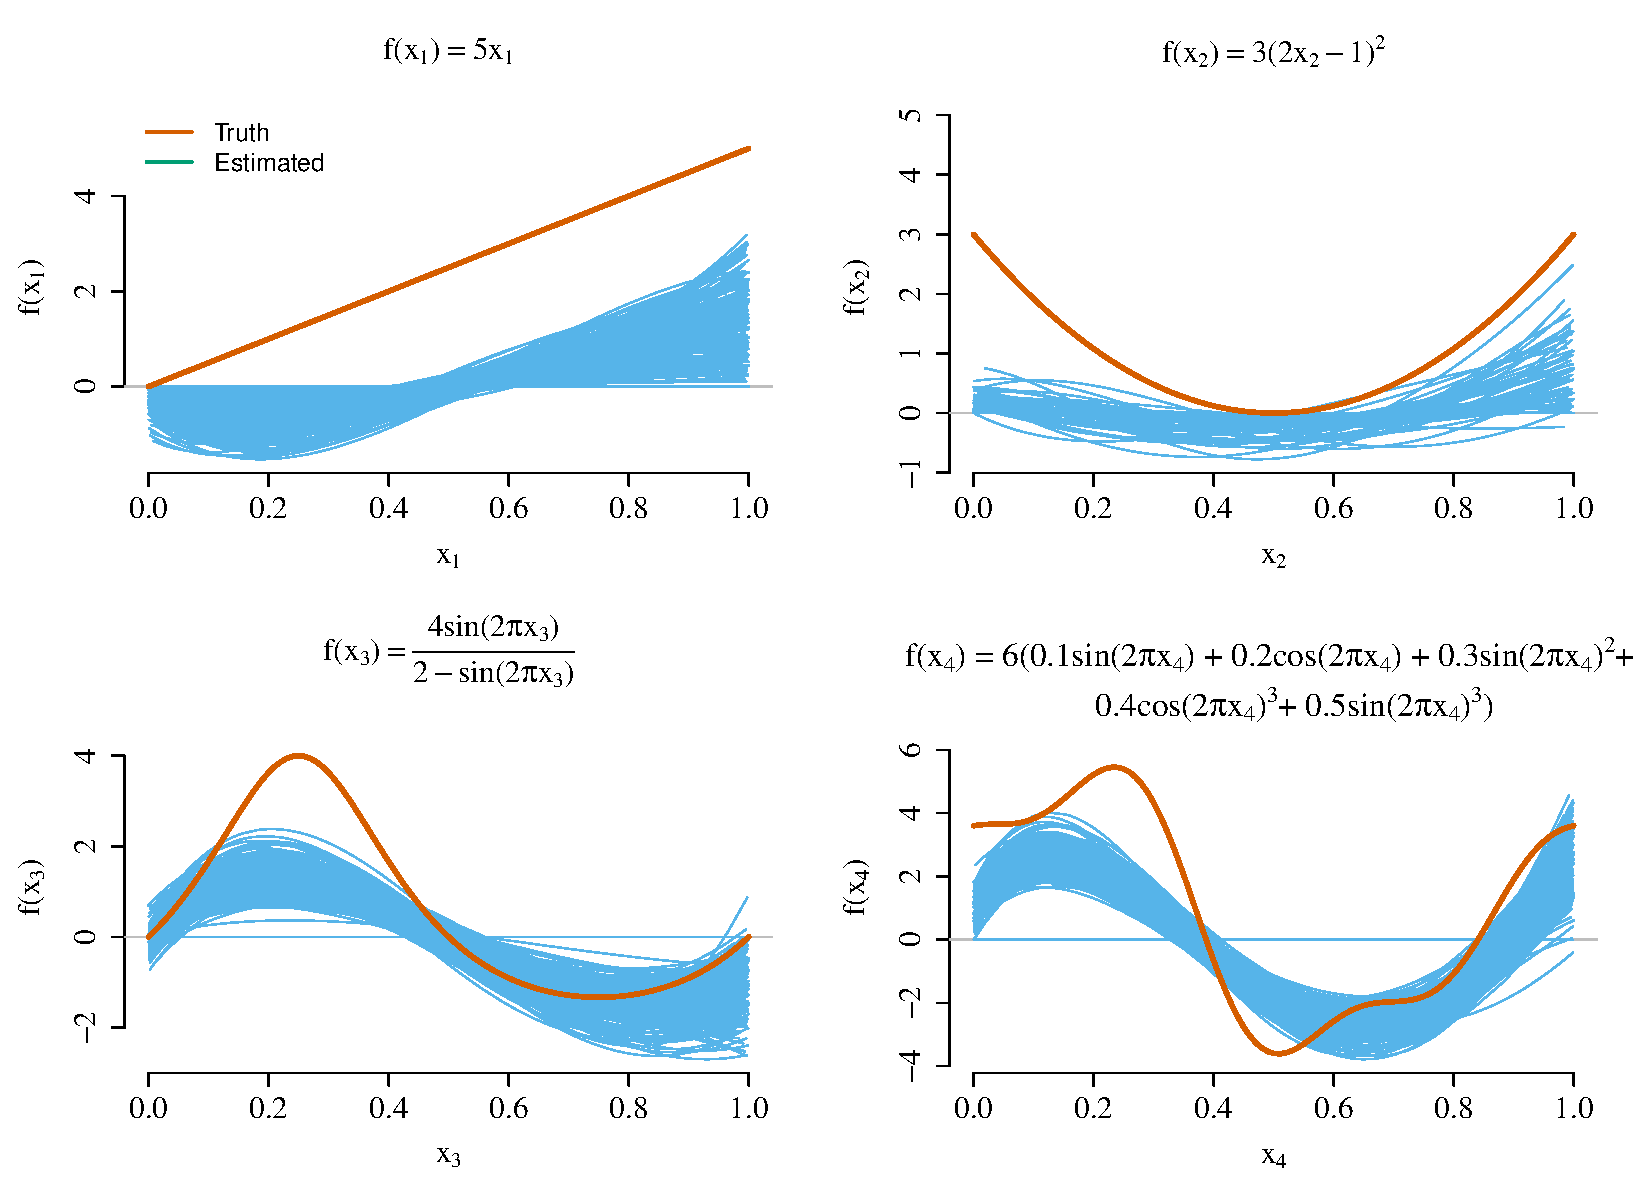
\includegraphics[scale=0.61]{figs/sail_main_eff_paramIndex1_200sims.pdf}
	\caption{True and estimated main effect component functions for scenario 1a). The estimated curves represent the results from each one of the 200 simulations conducted.}\label{fig:main_eff}
\end{figure}


\begin{figure}[H]
	\centering
	\subfloat{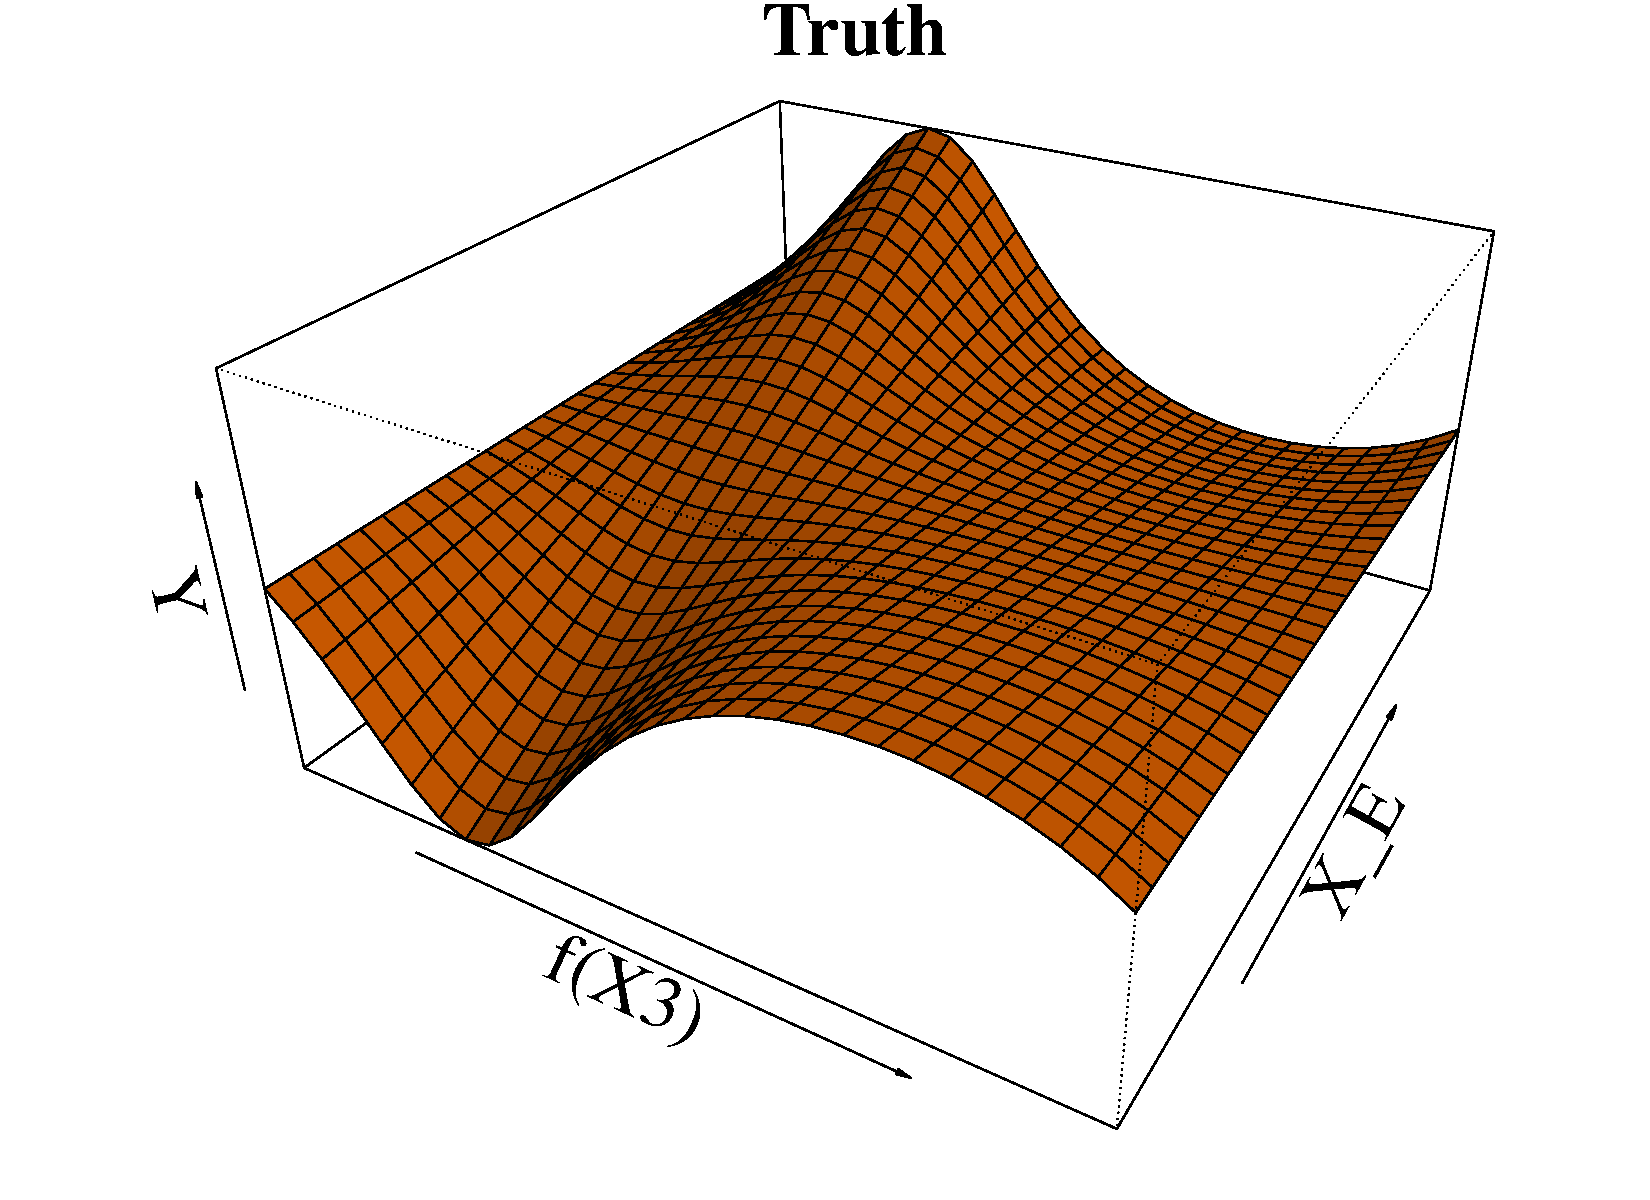
\includegraphics[width=0.37\linewidth]{figs/sail_intertruth_X3_paramIndex1_200sims.pdf}}
	\subfloat{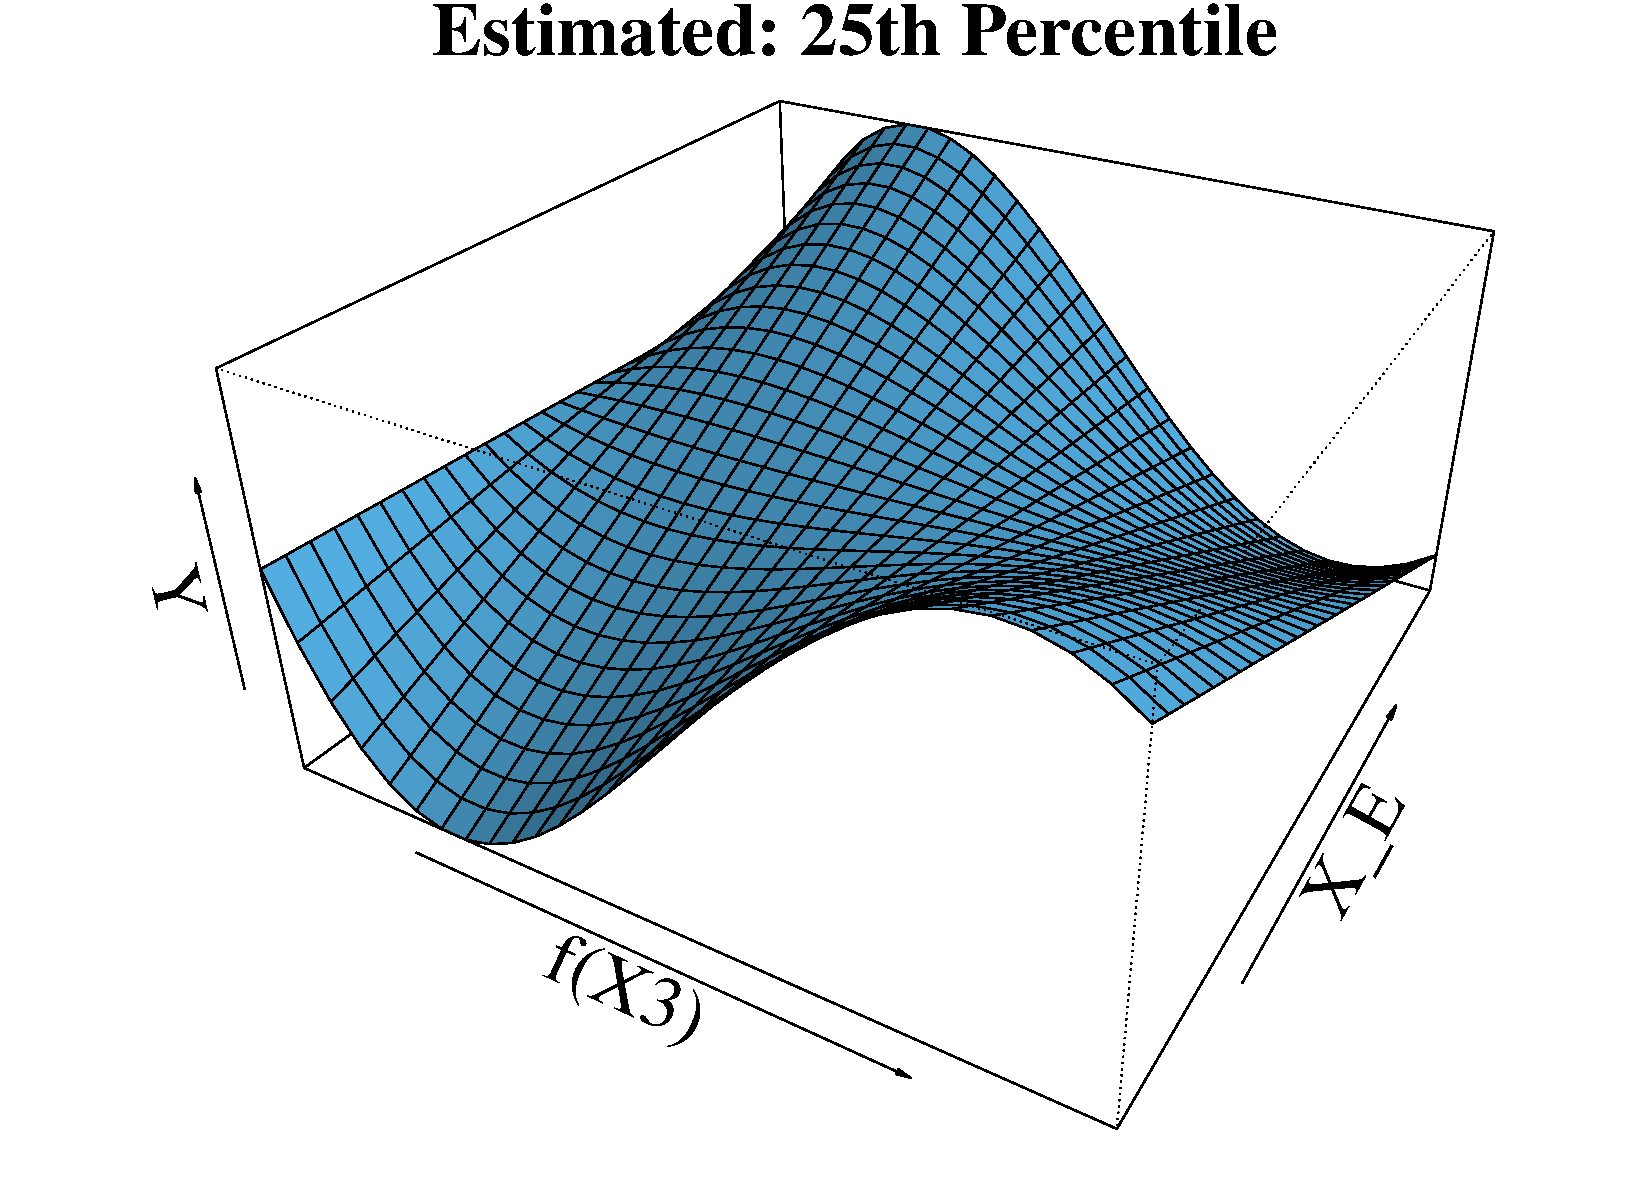
\includegraphics[width=0.37\linewidth]{figs/sail_inter25_X3_paramIndex1_200sims.pdf}}\quad 
	\subfloat{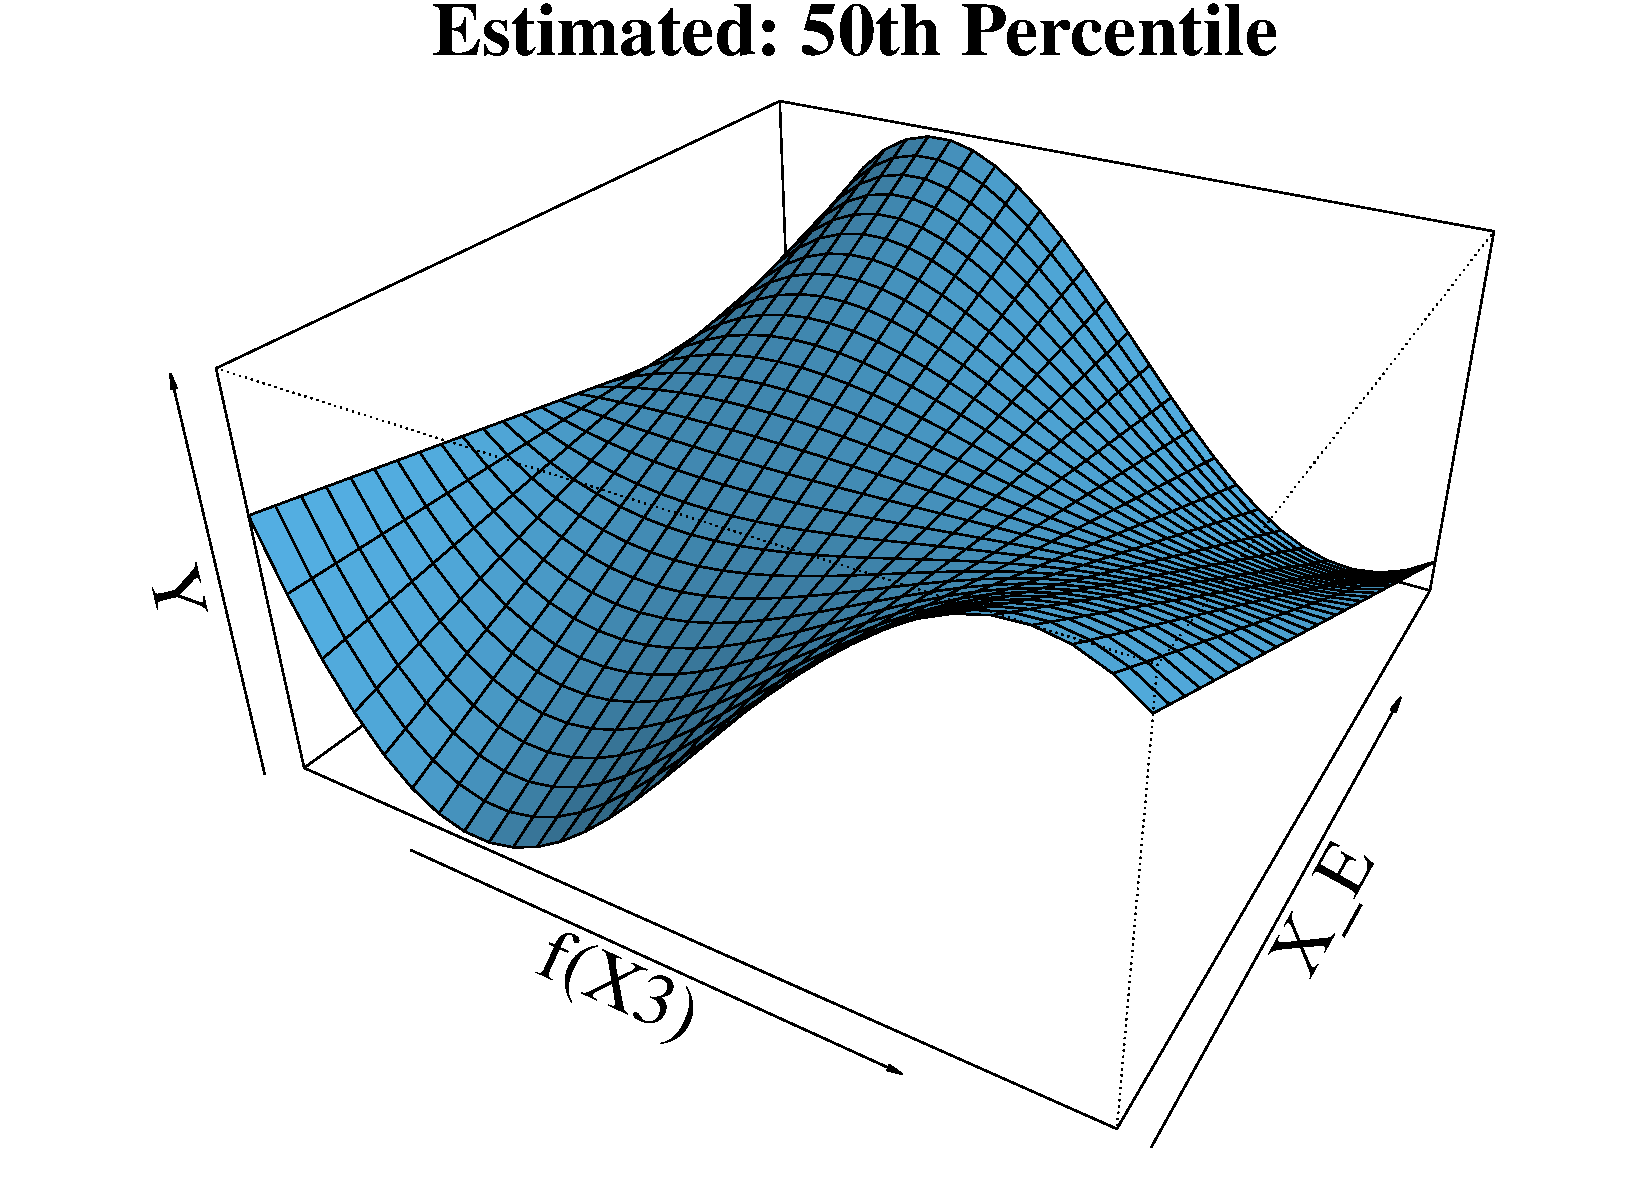
\includegraphics[width=0.37\linewidth]{figs/sail_inter50_X3_paramIndex1_200sims.pdf}}
	\subfloat{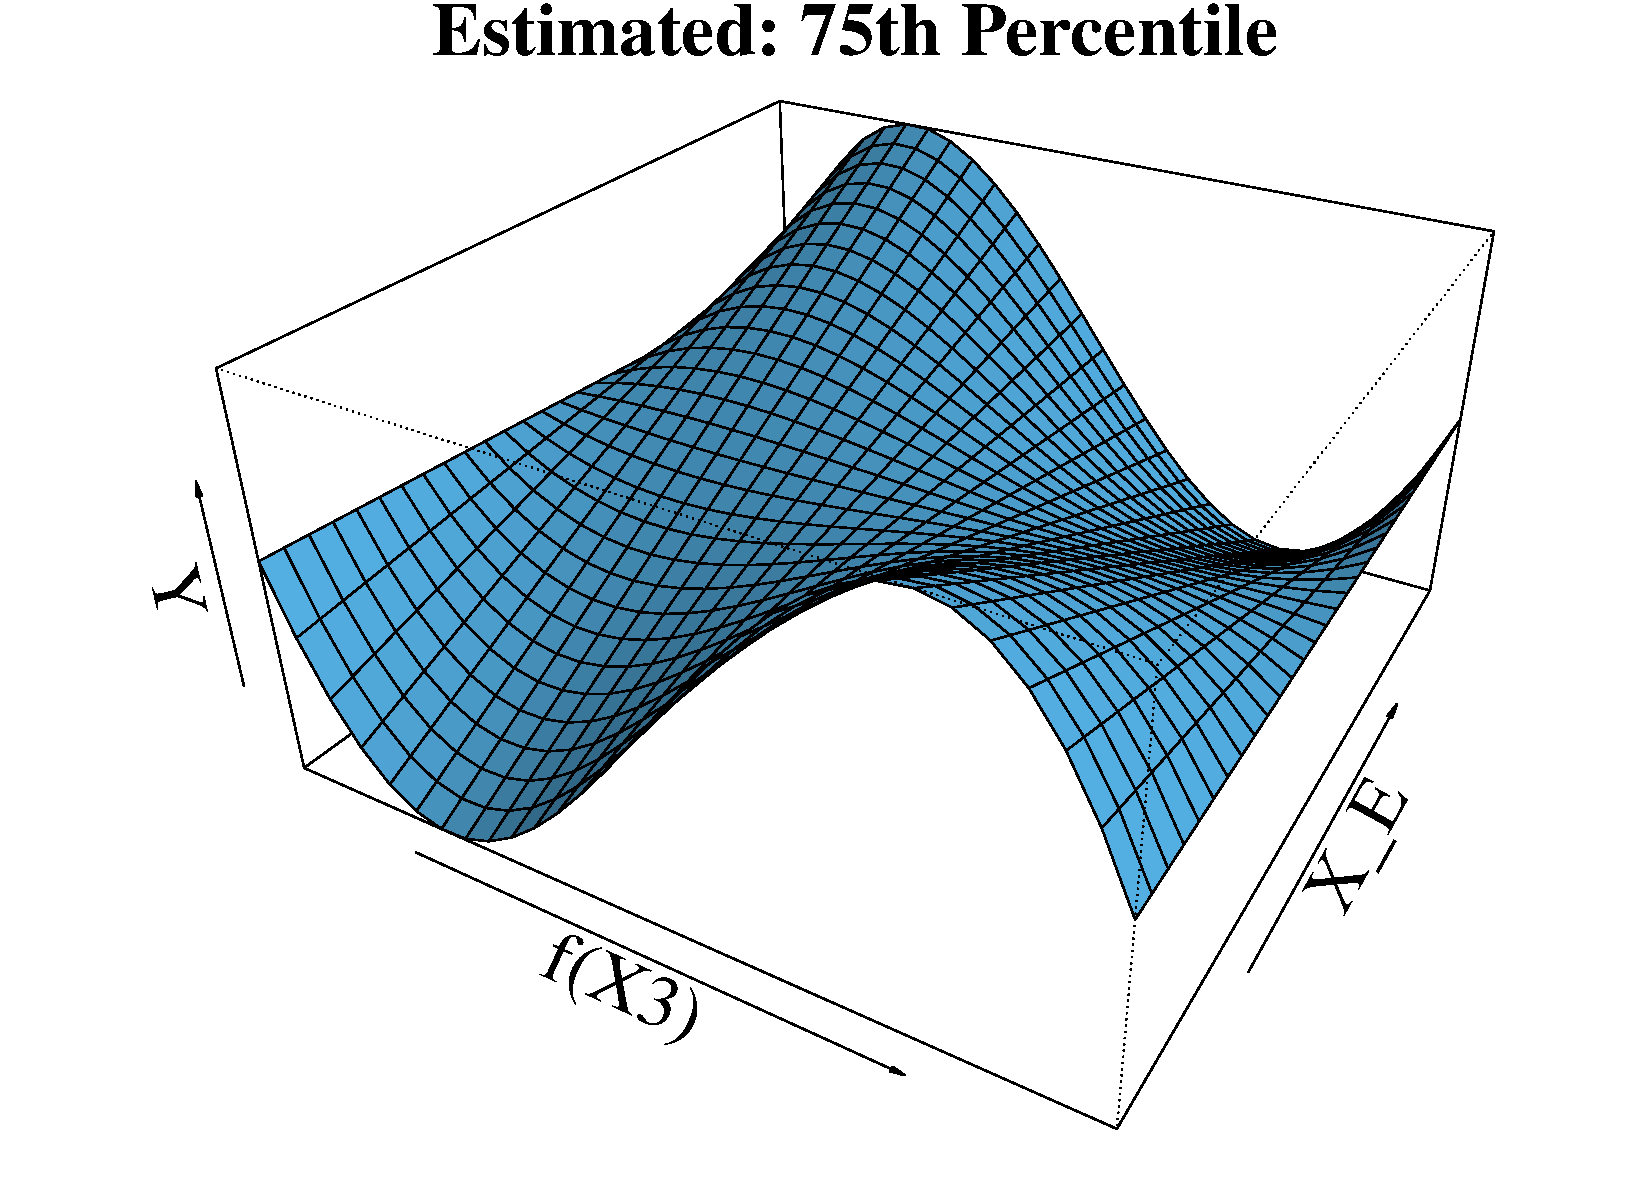
\includegraphics[width=0.37\linewidth]{figs/sail_inter75_X3_paramIndex1_200sims.pdf}}
	\caption{True and estimated interaction effects for $X_E \cdot f_3(X_3)$ in simulation scenario 1a).}
	\label{fig:X3}
\end{figure}


\begin{figure}[H]
	\centering
	\subfloat{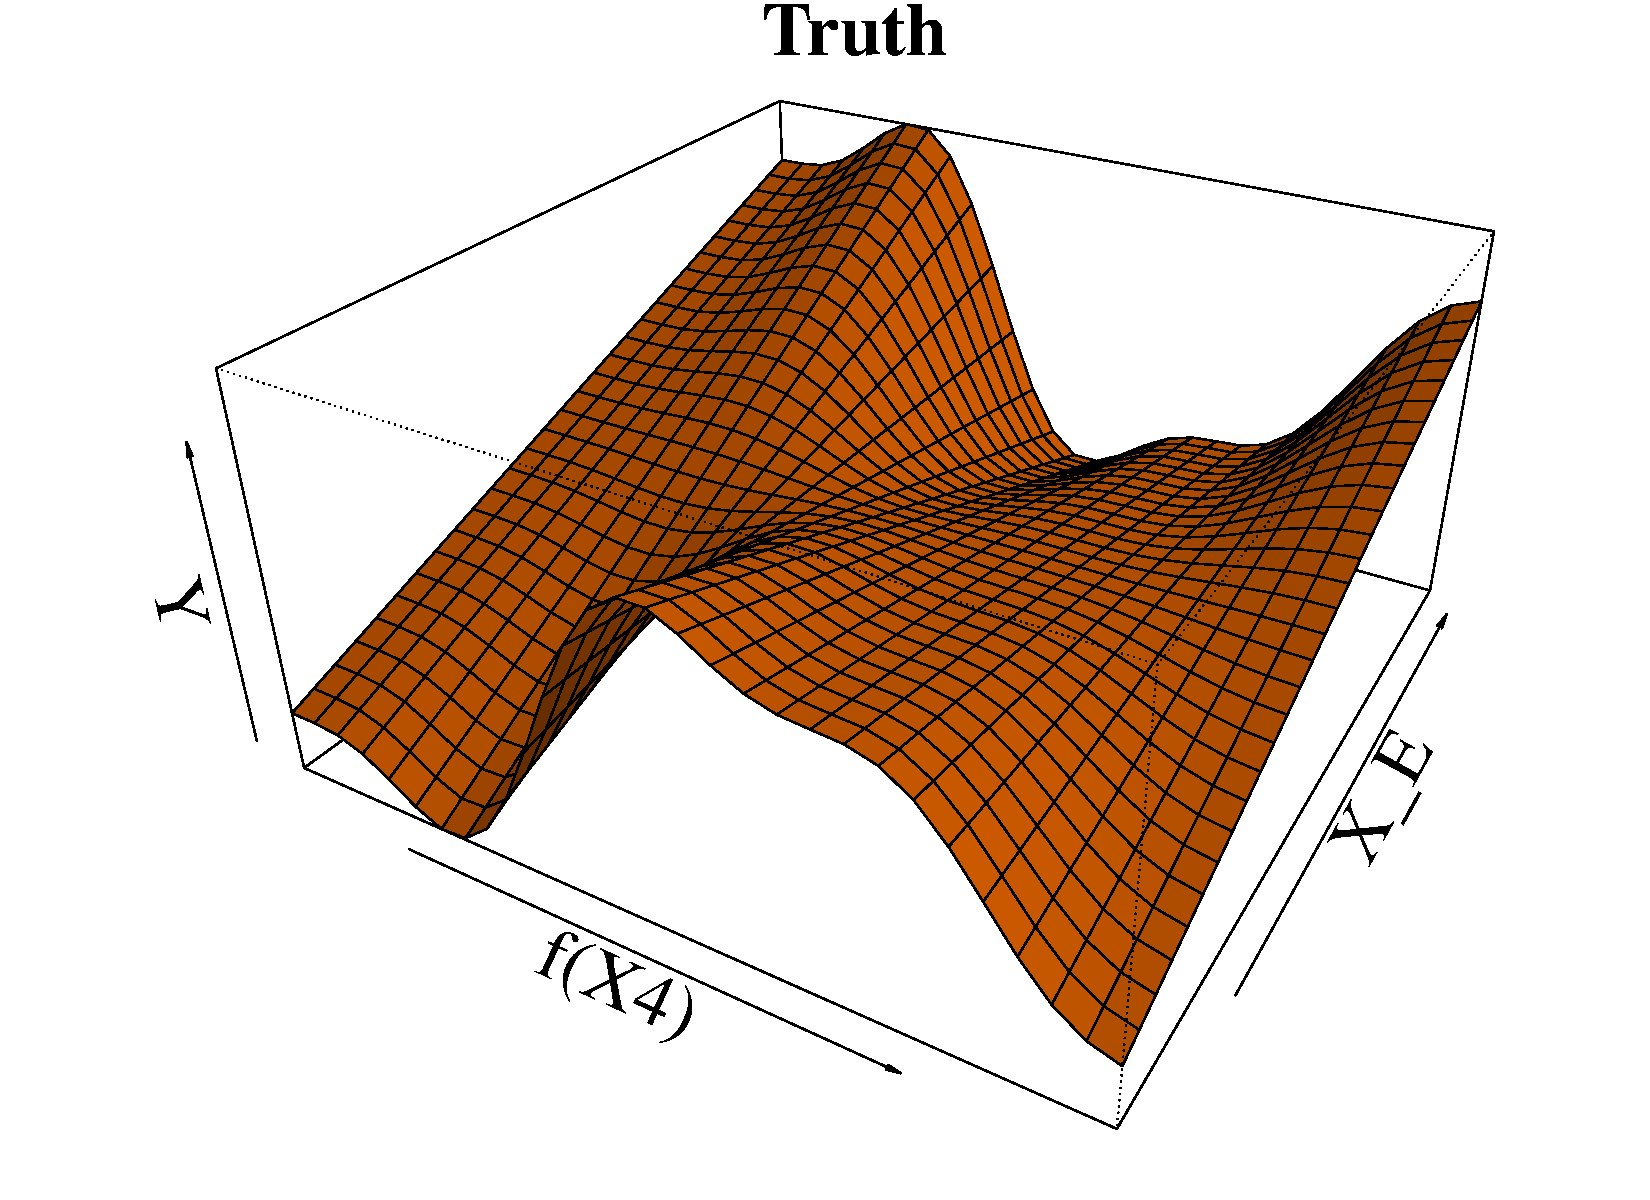
\includegraphics[width=0.37\linewidth]{figs/sail_intertruth_X4_paramIndex1_200sims.pdf}}
	\subfloat{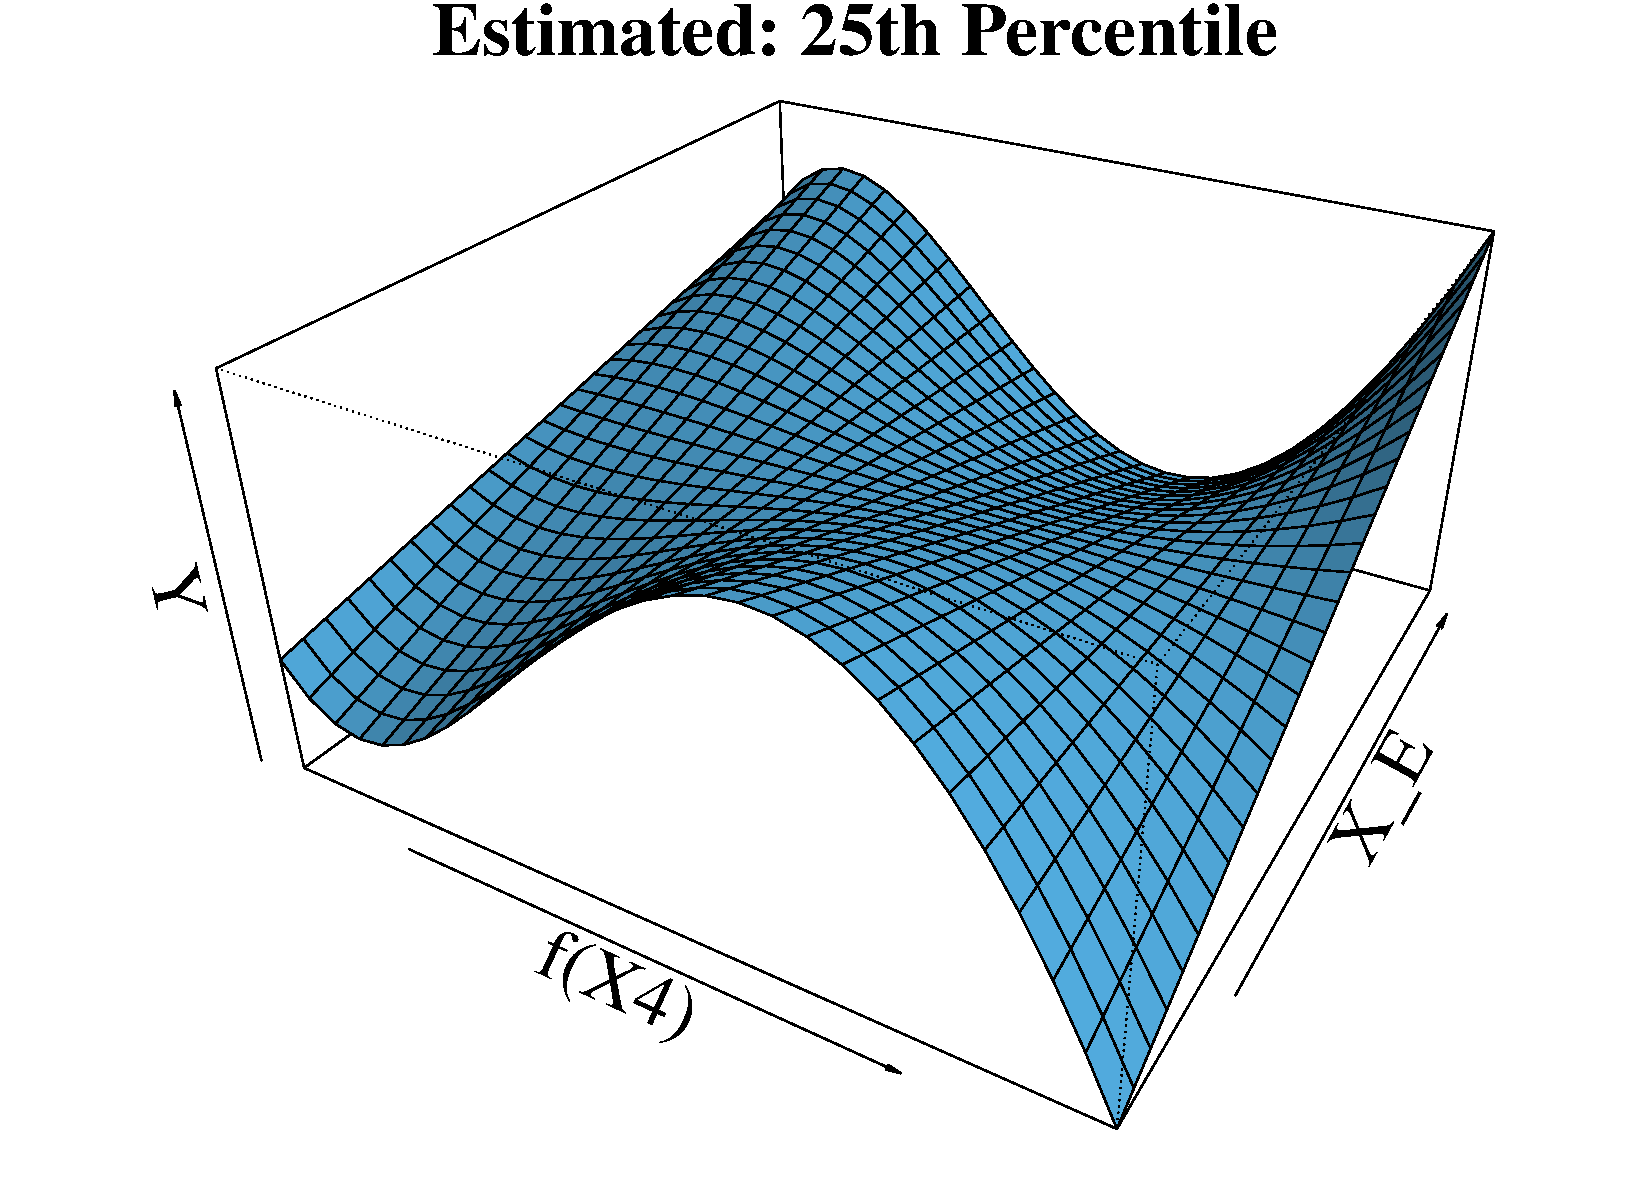
\includegraphics[width=0.37\linewidth]{figs/sail_inter25_X4_paramIndex1_200sims.pdf}}\quad 
	\subfloat{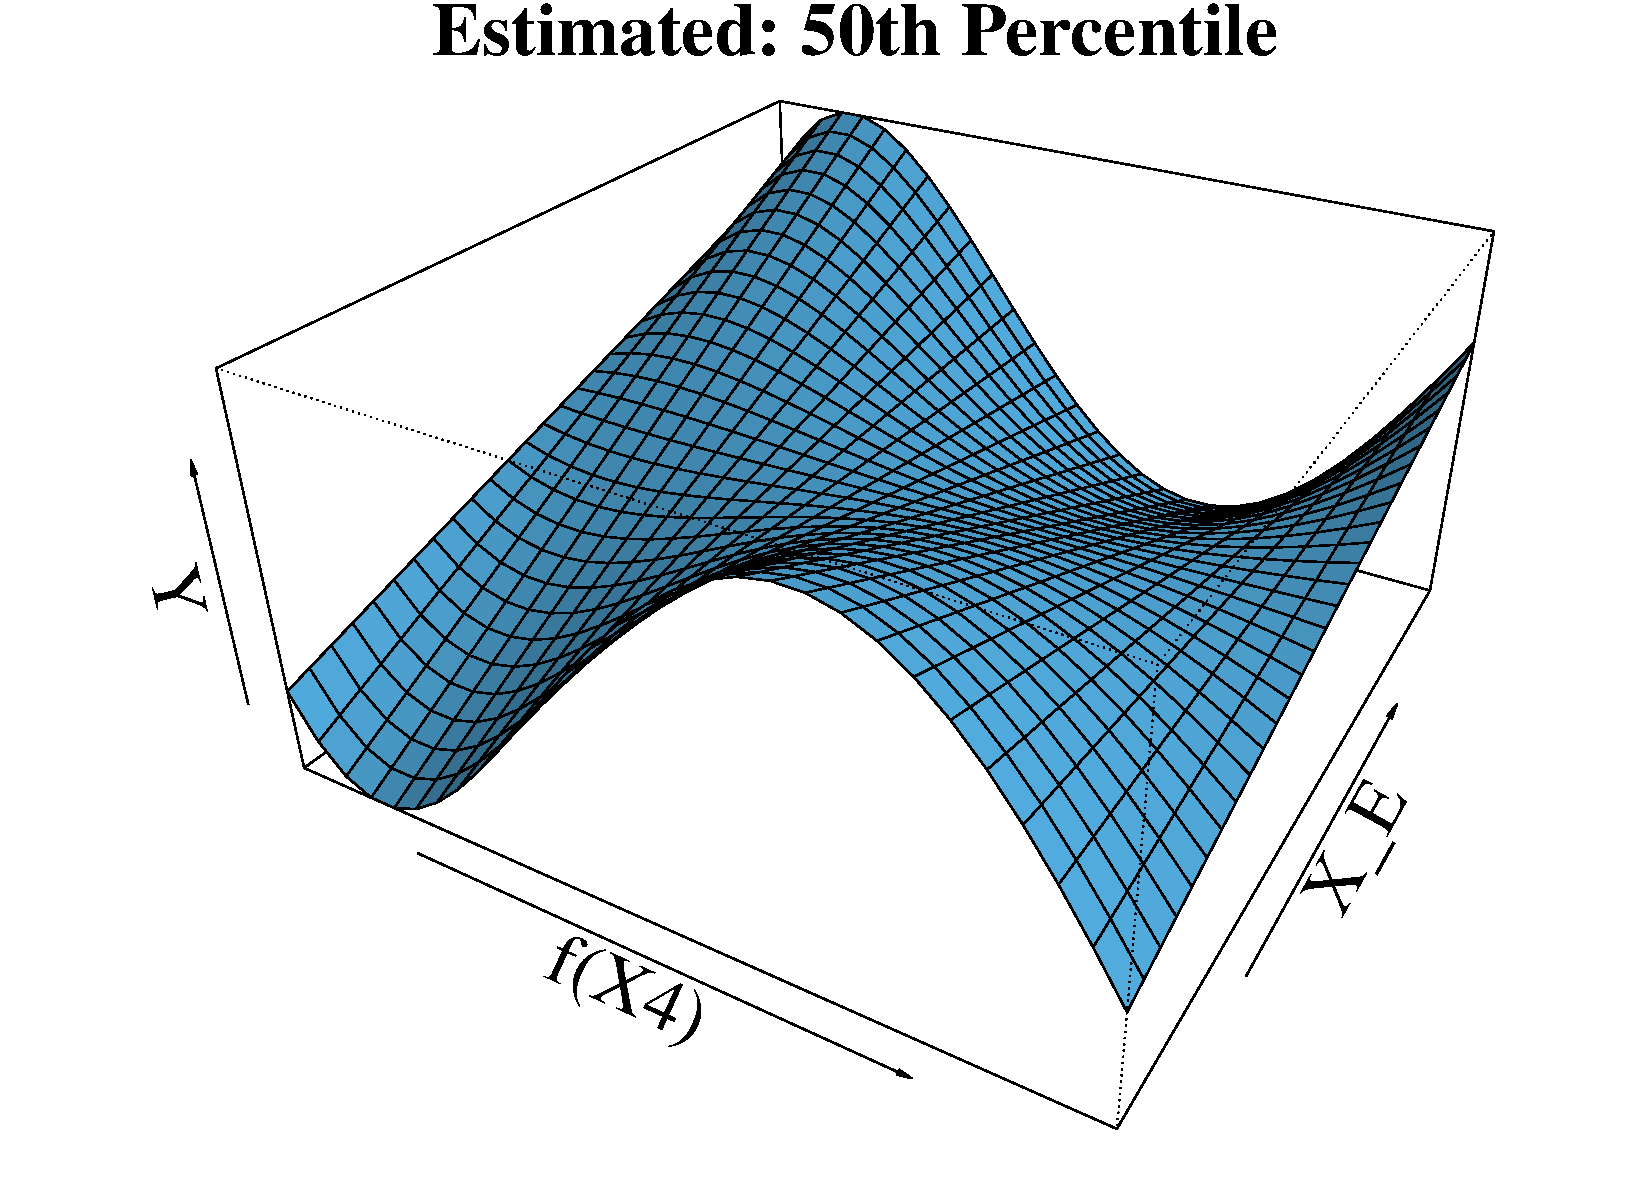
\includegraphics[width=0.37\linewidth]{figs/sail_inter50_X4_paramIndex1_200sims.pdf}}
	\subfloat{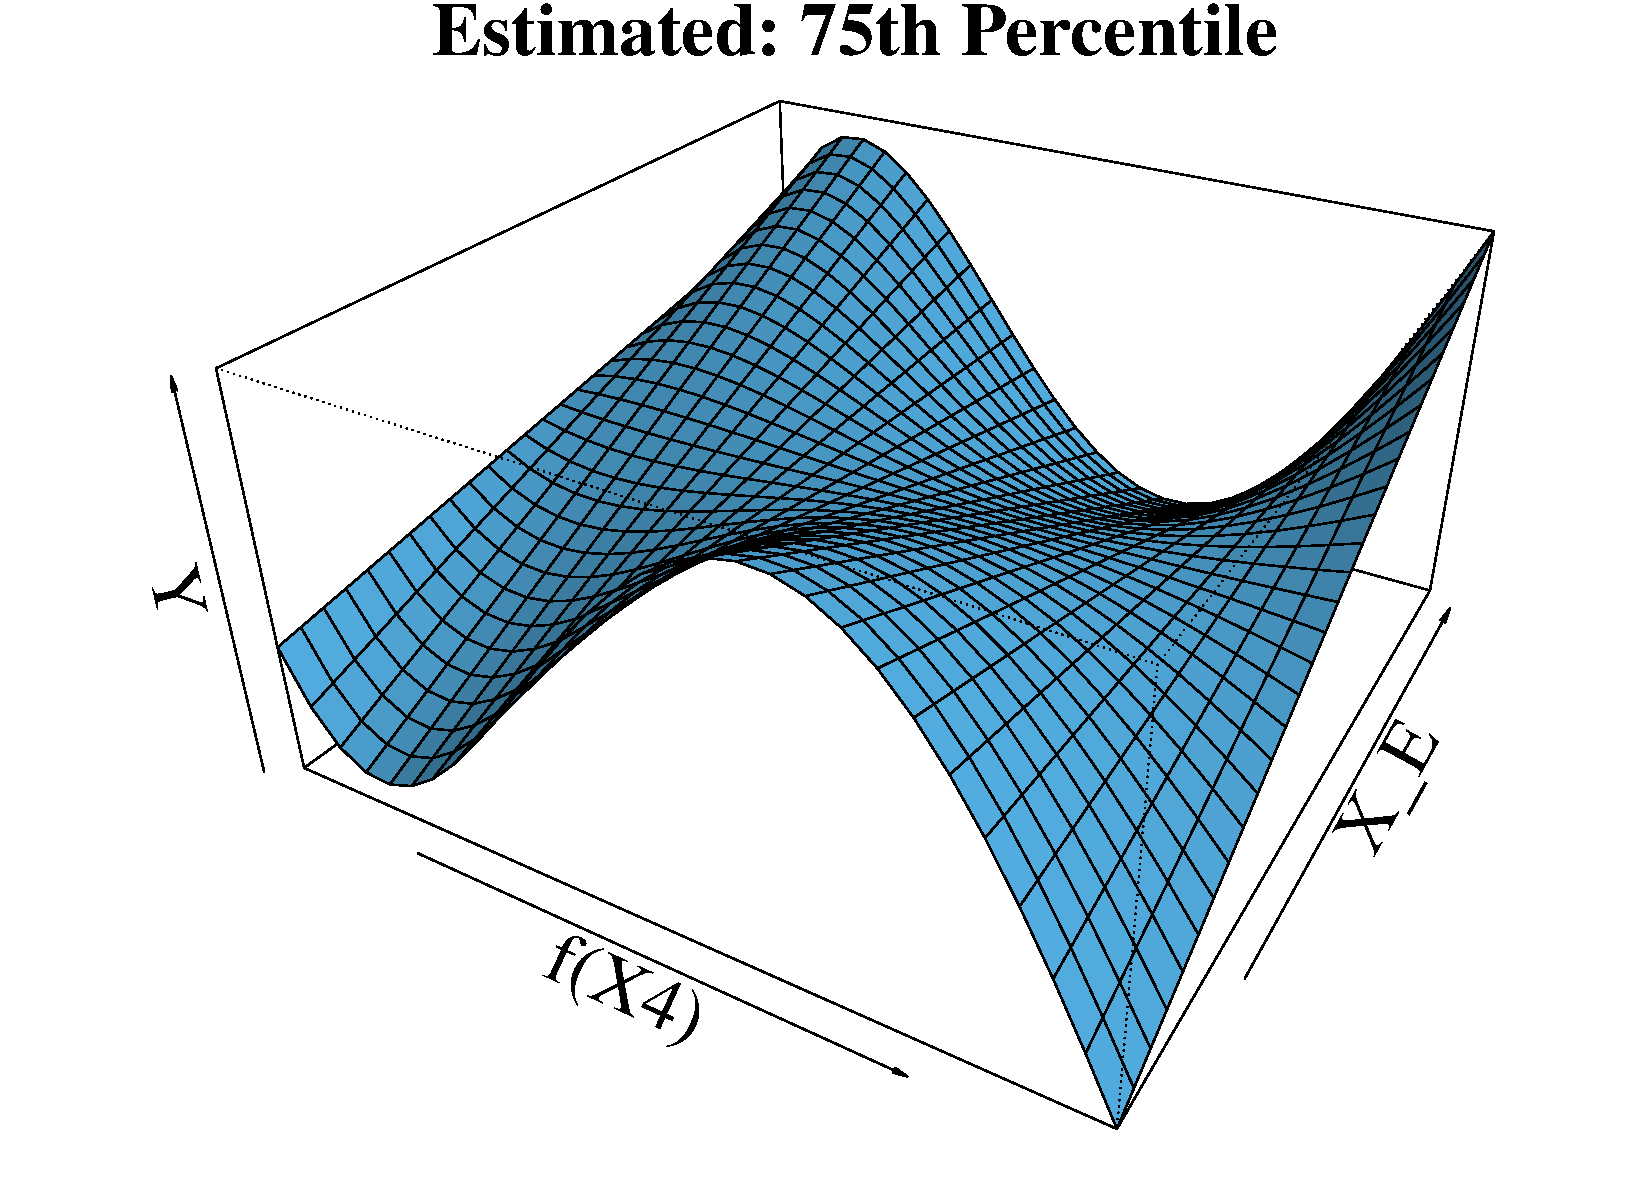
\includegraphics[width=0.37\linewidth]{figs/sail_inter75_X4_paramIndex1_200sims.pdf}}
	\caption{True and estimated interaction effects for $X_E \cdot f_4(X_4)$ in simulation scenario 1a).}
	\label{fig:X4}
\end{figure}


%\end{comment}


\section{Real Data Application with Alzheimer's Disease Neuroimaging Initiative} \label{sec:sail_rda}
%In this section we illustrate \sail ~on several real data examples.


%\subsection{Alzheimer's Disease Neuroimaging Initiative}

Alzheimer's is an irreversible neurodegenerative disease that results in a loss of mental function due to the deterioration of brain tissue. The overall goal of the Alzheimer's Disease Neuroimaging Initiative (ADNI) is to validate biomarkers for use in
Alzheimer's disease clinical treatment trials~\citep{petersen2010alzheimer}. The patients were selected into the study based on their clinical diagnosis: controls, \ac{mci} or \ac{ad}. PET amyloid imaging was used to asses \ac{amyb} protein load in 96 brain regions. The response we use here is general cognitive decline, as measured by a continuous mini-mental state examination score. We applied \sail ~to this data to see if there were any non-linear interactions between clinical diagnosis and A$\beta$ protein in the 96 brain regions on mini-mental state examination. 

There were a total of 343 patients who we divided randomly into equal sized training/validation/test splits. We ran the strong heredity \sail ~with cubic B-splines and $\alpha=0.1$. We also applied the \texttt{lasso, lassoBT, HierBasis} and \texttt{GLinternet} to this data. Using the same default settings and strategy as the simulation study, we ran each method on the training data, determined the optimal tuning parameter on the validation data, and assessed MSE on the test data. We repeated this process 200 times. 


\fig{error-crosses-adni-1}{error-crosses-adni}{16cm}{Mean test set MSE vs. mean number of active variables ($\pm 1$ SD) for ADNI data based on 200 train/validation/test splits.}{Mean test set MSE vs. mean number of active variables ($\pm 1$ SD) for ADNI data based on 200 train/validation/test splits.}

In Figure~\ref{fig:error-crosses-adni} we plot the mean test set MSE vs. the mean number of active variables $\pm 1$ SD. We see that \sail ~produces the sparsest models but doesn't perform as well as \texttt{HierBasis} and \texttt{GLinternet} in terms of MSE. \sail ~achieves a similar MSE to both the \texttt{lasso} and \texttt{lassoBT} with fewer variables on average. \texttt{GLinternet} produces the largest models and seems to be sensitive to the train/validate/test split as evidenced by the large standard deviations. 

To visualize the results from the \sail ~method, we chose the train/validate/test split which led to the best test set MSE, and then plotted the interaction effects in Figure~\ref{fig:plot-inter-adni}. The left panel shows the middle occipital gyrus left region in the occipital lobe known for visual object perception. We see that more A$\beta$ protein loads leads to a worse cognitive score for the MCI and AD group but not for the controls. The right panel shows the cuneus region which is known to be involved in basic visual processing, and we see that more A$\beta$ proteins leads to better cognitive scores for the MCI and AD group and poorer scores for the controls. 



\fig{plot-inter-adni-1}{plot-inter-adni}{16cm}{Estimated interaction effects by \texttt{sail} for the ADNI data.}{Estimated interaction effects by \texttt{sail} for the ADNI data.}




\section{Discussion} \label{sec:sail_discussion}

In this article we have introduced the sparse additive interaction learning model \sail ~for detecting non-linear interactions with a key environmental or exposure variable in high-dimensional settings. 
Using a simple reparametrization, we are able to achieve either the weak or strong heredity property without using a complex penalty function. We developed a blockwise coordinate descent algorithm to solve the \sail ~objective function for the least-squares loss function. 
%We show that the \texttt{adaptive sail} has the oracle property. 
All our algorithms are implemented in a computationally efficient, well-documented and freely available \texttt{R} package. 
Furthermore, our method is flexible enough to handle any type of basis expansion including the identity map, which allows for linear interactions. Our implementation allows the user to selectively apply the basis expansions to the predictors, allowing for example, a combination of continuous and categorical predictors. 
An extensive simulation study shows that \sail, \texttt{adaptive sail} and \texttt{sail weak} outperform existing penalized regression methods in terms of prediction error, sensitivity and specificity when there are non-linear main effects only, as well as interactions with an exposure variable. 

Our method however does have its limitations. \sail ~can currently only handle $X_E \cdot f(X)$ or $f(X_E) \cdot X$ and does not allow for $f(X, X_E)$, i.e., only one of the variables in the interaction can have a non-linear effect and we do not consider the tensor product. The reparametrization leads to a non-convex optimization problem which makes convergence rates difficult to assess, though we did not experience any major convergence issues in our simulations and real data analysis. The memory footprint can also be an issue depending on the degree of the basis expansion and the number of variables. 

To our knowledge, our proposal is the first to allow for non-linear interactions with a key exposure variable following the weak or strong heredity property in high-dimensional settings. We also provide a first software implementation for these models. 

\section*{Acknowledgements}
We thank Dr. Pedro Rosa-Neto for providing the ADNI data. 
